\newif\ifdebug
% \debugtrue
\newif\iffinal
% \finaltrue

% STRUCTURE AND LAYOUT

\documentclass[
	paper=a4,
	fontsize=13pt,
	open=any,
	headings=twolinechapter,
]{scrbook}


\newcommand{\notewidth}{4cm}
\newcommand{\notesep}{6mm}
\usepackage[
	\ifdebug showframe,\fi
	inner=20mm,
	marginparwidth=\notewidth,
	marginparsep=\notesep,
	outer=\dimexpr10mm + \notewidth + \notesep,
	bottom=4cm,
]{geometry}

\usepackage{layout}

\usepackage[strict]{changepage}
\newenvironment{fullwidth}
  {\begin{adjustwidth*}{}{\dimexpr-\marginparwidth-\marginparsep\relax}\vspace{-\baselineskip}}
  {\end{adjustwidth*}}


\usepackage{mparhack} % improved margin note positioning
\usepackage{sidenotes}

	% minimum vertical space between sidenotes
	\setlength\marginparpush{15pt}

	% make sidenote font size smaller
	% https://tex.stackexchange.com/q/361622/105570
	\makeatletter
	\RenewDocumentCommand\sidenotetext{ o o +m }{%	  
		\IfNoValueOrEmptyTF{#1}{%
			\@sidenotes@placemarginal{#2}{\textsuperscript{\thesidenote}{}~\footnotesize#3}%
			\refstepcounter{sidenote}%
		}{%
			\@sidenotes@placemarginal{#2}{\textsuperscript{#1}~#3}%
		}%
	}
	\makeatother

	% make sidenotes ragged
	% https://tex.stackexchange.com/a/359580/105570
	\makeatletter
	\RenewDocumentCommand \@sidenotes@placemarginal { m m }
	{
	  \IfNoValueOrEmptyTF{#1}
		{\marginpar[{\raggedleftmarginnote #2}]{\raggedrightmarginnote #2}}
		{\marginnote{#2}[#1]}%
	}
	\makeatother



% DEBUGGING

\usepackage{lipsum}
\usepackage{layout}

\newcommand{\toself}[1]{\iffinal\else\textcolor{blue}{\{\textsc{to self:} #1\}}\fi}
\newcommand{\todo}[1]{\iffinal\else\textcolor{purple}{\{\textsc{to do:} #1\}}\fi}
\newcommand{\urgent}[1]{\iffinal\else\textcolor{red}{\{\textsc{urgent:} #1\}}\fi}



% MATHEMATICS

\usepackage{quiver} % must precede {physics}
\usepackage{centernot}
\usepackage[
	math-style=ISO,
	warnings-off={mathtools-colon,mathtools-overbracket},
]{unicode-math}
\usepackage{physics}


\usepackage{mathtools}


\renewcommand{\op}[1]{{\operatorname{#1}}}

\DeclarePairedDelimiter{\ceil}{\lceil}{\rceil}
\DeclarePairedDelimiter{\floor}{\lfloor}{\rfloor}

\DeclareMathOperator{\arctanh}{arctanh}
% trig
\newcommand{\Co}{\mathrm{C}_}
\newcommand{\Si}{\mathrm{S}_}
\newcommand{\Ta}{\mathrm{T}_}



% Set builder notation (usage: `\set{a | P(a)}` or `\set[\big]{1, 2}`)
\usepackage{xparse}
\usepackage{ifthen}
\DeclarePairedDelimiterX{\setdelim}[1]{\{}{\}}{\setargs{#1}}
\NewDocumentCommand{\setargs}{>{\SplitArgument{1}{|}}m}{\setargsaux#1}
\NewDocumentCommand{\setargsaux}{mm}{\IfNoValueTF{#2}{#1}{#1\nonscript\:\delimsize\vert\allowbreak\nonscript\:\mathopen{}#2}}%
\newcommand{\set}[2][*]{\ifthenelse{\equal{\detokenize{#1}}{*}}{\setdelim*{#2}}{\setdelim[#1]{#2}}}


% quaternions
\newcommand{\ii}{\vb{\skew{1}\hat{\clipbox{0pt 0pt 0pt 2.7pt}{$i$}} }}
\newcommand{\jj}{\vb{\skew{3}\hat{\clipbox{0pt 0pt 0pt 2.7pt}{$j$}} }}
\newcommand{\kk}{\vb{\hat k}}


% basis vectors
\renewcommand{\vb}[1]{\symbfit{#1}}
\newcommand{\ve}{\vb{e}}
\newcommand{\vg}{\vb{γ}}
\newcommand{\vs}{\vec{σ}}
\newcommand{\dx}{\dd x}
\newcommand{\∂}{\symbf{∂}}

\newcommand{\spanof}{\op{span}\set}

\renewcommand{\ip}[1]{\left⟨ #1 \right⟩}

% special structures
\newcommand{\manif}{\mathcal}	% manifold
\newcommand{\cat}{\mathbf}	% category
\newcommand{\liealg}{\mathfrak}	% Lie algebra
\newcommand{\lin}{\mathrm}	% linear map
\newcommand{\rotor}{\mathscr}	% geometric algebra rotors

% fields
\usepackage{dsfont}
\newcommand{\FF}{\mathds{F}}
\newcommand{\RR}{\mathds{R}}
\newcommand{\CC}{\mathds{C}}
\newcommand{\HH}{\mathds{H}}
\newcommand{\ZZ}{\mathds{Z}}
\newcommand{\NN}{\mathds{N}}

% groups
\DeclareMathOperator{\SO}{SO}
\DeclareMathOperator{\GL}{GL}

% quotient structure
\newcommand{\quot}[3][*]{
	\if*#1
		\left. #2 \middle/ #3 \right.
	\else
		#2 #1/ #3
	\fi
}

% generator
\newcommand{\gen}[1]{\set{\!\set{#1}\!}}

% transpose superscript
\newcommand{\transpose}{^{\mkern-1.5mu\mathsf{T}}}


% path-ordered exponential
\newcommand{\Pexpl}[1][]{\accentset{←}{\mathds{P}}_{#1}\exp}
\newcommand{\Pexpr}[1][]{\accentset{→}{\mathds{P}}_{#1}\exp}


% algebras
\newcommand{\TA}[2][]{{#2}^{⊗#1}}
\usepackage{scalerel}
\newcommand{\EA}[1][]{\scalerel*{\wedge}{V}^{#1}}
\newcommand{\SA}[1][\,]{𝒮^{\!#1}}
\newcommand{\GA}[1][]{𝒢_{#1}}

\newcommand{\forms}[1][]{\op{Ω}^{#1}}


% shortcuts

% easy dotted sequence: \etc{𝒖_{\i}}{⊗}{k} → 𝒖_1 ⊗ ··· ⊗ 𝒖_k
\newcommand{\etc}[4][1]{
	{\def\i{#1} #2}
	#3 \if,#3 \dots \else \cdots \fi #3
	{\def\i{#4} #2}
}
\newcommand{\etcskip}[5][1]{
	{\def\i{#1} #2}
	#3 \if,#3 \dots \else \cdots \fi #3
	{\def\i{#4} \widehat{#2}}
	#3 \if,#3 \dots \else \cdots \fi #3
	{\def\i{#5} #2}
}
\newcommand{\etcmid}[5][1]{
	{\def\i{#1} #2}
	#4 \if,#4 \dots \else \cdots \fi #4
	{#3}
	#4 \if,#3 \dots \else \cdots \fi #4
	{\def\i{#5} #2}
}


\makeatletter
\newcommand{\sig}[1]{(\@tfor\elem:=#1\do{{\elem}})}
\makeatother




% geometric algebra
\DeclarePairedDelimiter{\angbr}{⟨}{⟩}
\newcommand{\grade}[2][]{\angbr*{#2}_{#1}}

\newcommand{\vol}{\mathds{I}}

\newcommand{\rev}[1]{#1^\dagger}
\newcommand{\revsign}[1]{s_{#1}}

\newcommand{\invol}[1]{#1^\star}

\newcommand{\bch}[2]{#1 \odot #2}

% self-reverse and anti-self-reverse projections
\newcommand{\srev}[1]{\qty{\!\!\qty{#1}\!\!}}
\newcommand{\arev}[1]{\qty[\!\qty[#1]\!]}

% "fat dot" product
% https://tex.stackexchange.com/a/235120/105570
\makeatletter
\newcommand*\fatdot{\mathpalette\bigcdot@{.8}}
\newcommand*\bigcdot@[2]{\mathbin{\vcenter{\hbox{\scalebox{#2}{$\m@th#1\bullet$}}}}}
\makeatother

\newcommand{\wedot}{\mathrel{\ooalign{\hfil$∧$\hfil\cr\hfil$.$\hfil}}}

% left and right contractions
\newcommand{\lcontr}{\mathrel{\rfloor}}
\newcommand{\rcontr}{\mathrel{\lfloor}}






% DIFFERENTIAL GEOMETRY


% topological sphere
\newcommand{\Sphere}{\mathscr{S}}


% tangent bundle, vertical bundle
\DeclareMathOperator{\TT}{T}
\DeclareMathOperator{\VV}{V}

% section of bundle
\DeclareMathOperator{\secs}{Γ}

% injection, surjection, bijection
\newcommand{\inject}{\hookrightarrow} % ↪︎
\newcommand{\surject}{\twoheadrightarrow} % ↠
\usepackage{trimclip}
\newcommand{\biject}{\mathrel{%
\mathrlap{\clipbox*{0 -1ex {0.5\width} {\height}}{$\inject$}}%
\surject}}

% fibre bundle A ↪︎ B ↠ C
\newcommand{\fibrebundle}[4][]{#2 \inject #3 \overset{#1}{\surject} #4}


% transport operator
\newcommand{\trans}{\operatorname{trans}\displaylimits}


% derivatives
\DeclareMathOperator{\DD}{D}
\newcommand{\vd}{\symbf{∂}}
\newcommand{\VD}{\symbfcal{D}}
\newcommand{\bd}{\symbfup{d}}

\newcommand{\lie}{\pounds}

% explicit differential form
\usepackage{accents}
\newcommand{\df}[1]{\underaccent{\sim}{#1}}



\usepackage{amsthm}
	\newtheorem{definition}{Definition}
	\newtheorem{theorem}{Theorem}
	\newtheorem{lemma}{Lemma}
	\newtheorem{corollary}{Corollary}
	\newtheorem{proposition}{Proposition}


% TYPOGRAPHY

\setmainfont{Libertinus Serif}
% \setsansfont{Libertinus Sans}

\iffalse
\setmathfont{Libertinus Math}
\else
\setmathfont{latinmodern-math.otf}
\setmathfont[range=\varnothing]{Libertinus Math}
\fi

\linespread{1.07}

\newcommand{\textdef}{\textsc}

\usepackage{testhyphens}
\hyphenation{
	auto-morph-ism
	auto-morph-isms
	anti-auto-morph-ism
	anti-auto-morph-isms
}

% correct hyphenation for parenthesised prefixes.
\newcommand{\paren}[1]{(#1\discretionary{-)}{}{)}\nolinebreak\hspace{0pt}}
% Usage: \paren{anti}disestablishment produces hyphenation like:
% (anti)disestablishment (anti-) %
% disestablishment (anti)disest- %
% ablishment...


\usepackage{caption}
\setcapindent{0pt} % remove indentation for multiline (table) captions
\captionsetup{font=footnotesize}

\usepackage{enumitem}



% FIGURES

\newcommand{\includefigure}[2][\columnwidth]{
	\graphicspath{{figures/}}
	\def\svgwidth{#1}
	\input{figures/#2.pdf_tex}
}



% REFERENCING

\usepackage[numbers,sort&compress]{natbib}
\bibliographystyle{my-thesis-style}
\usepackage{doi}

\usepackage{xcolor}
\usepackage{hyperref}
	\hypersetup{
		colorlinks,
		linkcolor={red!50!black},
		urlcolor={blue!60!black},
		citecolor={green!50!black},
	}

\usepackage{cleveref}

% AUTONUM HACKS %
	% supress dumb warning
	% https://tex.stackexchange.com/a/285953/105570
	\let\globcount\newcount
	\expandafter\def\csname ver@etex.sty\endcsname{3000/12/31}
\usepackage{autonum}
	% make \Cref work as well as \cref
	% https://tex.stackexchange.com/a/471654/105570
	\makeatletter
	\autonum@generatePatchedReferenceCSL{Cref}
	\makeatother




\title{Geometric Algebra for Special and General Relativity}
\author{Joseph Wilson}

\begin{document}


% FRONT MATTER
\newgeometry{margin=3.5cm} % begin front matter

	\maketitle
	\tableofcontents

\restoregeometry % end front matter

\ifdebug
	\layout

\setcounter{chapter}{-1}
\chapter{Proof of Document Features}

\section{Referencing}

\subsection{Automatic equation labels}
Unlabelled, unreferenced:
\begin{equation}
	a^2 = π
\end{equation}
Labelled, unreferenced:
\begin{equation}
	\label{eqn:1}
	b^2 = ρ
\end{equation}
Labelled, referenced:
\begin{equation}
	\label{eqn:2}
	c^2 = σ
\end{equation}
See \cref{eqn:2}.

\subsection{Reference naming}
Suppose
\begin{equation}
	\label{eqn:3}
	d^2 = η
.\end{equation}
\Cref{eqn:3} proves.
\begin{theorem}[Diogenes]
	\label{thm:1}
	Something.
\end{theorem}
By \cref{thm:1}, something. \Cref{thm:1} states something.
\begin{definition}
	\label{def:1}
	Deduction.
\end{definition}
See \cref{def:1}. \Cref{def:1} defines.
\begin{lemma}
	\label{lem:1}
	Little.
\end{lemma}
A small result is \cref{lem:1}. \Cref{lem:1} is nice.


\section{Side margins}

\lipsum[1][1-6]\sidenote{
	This is a long sidenote on two lines.
}
\lipsum[2][1-3]\sidenote{
	\lipsum[4][1-4]
}
\lipsum[3][1]\sidenote{
	Does this fit?
}
\lipsum[3][2-4]

\section{Links and citations}

This is a \url{http://url.com}.
A like to think this will turn out OK \cite{misner1973gravitation}.
All my inspiration is from \cite{gallian2021abstract-algebra,spivak1975dg,lee2012diffgeo}.


\section{Mathematical macros}

Set builders:
\begin{align}
	\varnothing, \set{}, \set{1}, \set{1, 9\frac34}, \set{x^2 | x ∈ \RR}
\end{align}
Custom sizing:
\begin{align}
	\set[\bigg]{1}, \set[]{\int}
\end{align}
Misc.
\begin{align}
	\grade[p]{A + B}, \TA{(\TT^*ℳ)}, \EA[k]{V}, \SA{\RR^n}, \GA[2](V, η)
\end{align}


\section{Hyphenation}

\paren{anti}automorphism \paren{anti}automorphism \paren{anti}automorphism \paren{anti}automorphism \paren{anti}automorphism \paren{anti}automorphism \paren{anti}automorphism \paren{anti}automorphism \paren{anti}automorphism \paren{anti}automorphism \paren{anti}automorphism \paren{anti}automorphism.
\lipsum[1][1]
\paren{anti}automorphism \paren{anti}automorphism \paren{anti}automorphism \paren{anti}automorphism \paren{anti}automorphism \paren{anti}automorphism \paren{anti}automorphism \paren{anti}automorphism \paren{anti}automorphism.

\begin{checkhyphens}
	neighbourhood
	neighbourhoods
	automorphism
	automorphisms
\end{checkhyphens}
\fi





\part{Special Relativity and Geometric Algebra}
\label{part:1}

\chapter{Introduction}

The Special Theory of Relativity is a model of \emph{spacetime} --- the geometry in which physical events take place.
Spacetime comprises the Euclidean dimensions of space and time, but only in a way relative to each observer moving through it: there exists no single `universal' ruler or clock.
Instead, two observers in relative motion define different decompositions of spacetime, and their respective clocks and rulers are found to disagree according to the Lorentz transformation laws.
The insight of special relativity is that one should focus not on the observer-dependent notions of space and time, but on the Lorentzian geometry of spacetime itself.

Seven years after Albert Einstein introduced this theory,\sidenote{
	Einstein’s paper \cite{einstein1905electrodynamics} was published in 1905, the so-called \emph{Annus Mirabilis} or ``miracle year'' during which he also published on the photoelectric effect, Brownian motion and the mass-energy equivalence.
	Each of the four papers was a monumental contribution to modern physics.
} he succeeded in formulating a relativistic picture which included gravity.
In this General Theory of Relativity, gravitation is identified with the curvature of spacetime over astronomical distances.
Both theories coincide locally when confined to sufficiently small extents of spacetime, over which the effects of curvature are negligible.
In \cref{part:1}, we will focus on special relativity, leaving gravity and curvature to \cref{part:2}.

From the Erlangen programme,\sidenote{
	Introduced by Felix Klein in 1872 \cite{klein1893erlangen}, the Erlangen program characterises geometries (Euclidean, hyperbolic, projective, etc.) by their symmetry groups and invariants.
	E.g., Euclidean geometry studies the invariants of rigid transformations.
} the study of local spacetime geometry amounts to the study of its intrinsic symmetries.
These symmetries form the Poincaré group, and consist of spacetime translations and Lorentz transformations, the latter being the extension of the rotation group for Euclidean space to relativistic rotations of spacetime.
The standard matrix representation of the Lorentz group, $\SO^+(1, 3)$, is the connected component of the orthogonal group
\begin{align}
	\op{O}(1,3) = \set{\lin Λ ∈ \GL(\RR^4) | \lin Λ\trans\lin η\lin Λ = \lin η}
\end{align}
with respect to the bilinear form $η = ±\op{diag}(-1,+1,+1,+1)$.
The rudimentary tools of matrix algebra are sufficient for an analys the Lorentz group, and are familiar to any physicist.

However, the last century has seen many other mathematical tools be applied to the study of generalised rotation groups such as $\SO^+(1,3)$ or the rotation group $\SO(3)$ of $\RR^3$.
Among these tools is the \emph{geometric algebra}, invented\sidenote{
	Clifford algebra was independently discovered by Rudolf Lipschitz two years later \cite{lipschitz1880clifford-alg}. 
	He was the first to use them to the study the orthogonal groups.
} by William Clifford in 1878 \cite{clifford1878grassmann}.
Geometric algebra remains largely unknown in the physics community, despite arguably being far superior for the description of rotations than traditional matrix techniques.
It is good to glean some of the history that led to this (perhaps unfortunate) state of the field.

\subsubsection{The quest for an optimal formalism for rotations}

Mathematics has seen the invention of a variety of vector formalisms since the 1800s, and the question of which is best suited to physics has a long contentious history.

Complex numbers had been known for a long time\sidenote{
	Since Wessel, Argand and Gauss in the 1700s \cite{chappell2016quat-history}.
} to be useful descriptions of planar rotations.
William Hamilton's efforts to extend the same ideas into three dimensions by inventing a ``multiplication of triples'' bore fruition in 1843, when the quaternion algebra
\begin{align}
	\ii^2 = \jj^2 = \kk^2 = \ii\jj\kk = -1
\end{align}
came to him in revelation.
In following decades, William Gibbs developed the vector calculus of $\RR^3$ with the usual vector cross and dot products.
The ensuing vector algebra ``war'' of 1890--1945 saw Hamilton's prized\sidenote{
	Hamilton had dedicated following in the time that quaternions were in fasion: the \emph{Quaternion Society} existed from 1895 to 1913.
} quaternion algebra $\HH$, hailed as the optimal tool for describing $3$d rotations, struggle for popularity against Gibbs' easier-to-visualise vector calculus.
Today, quaternions are generally regarded in physics as an old-fashioned mathematical curiosity.


\todo{...introduce}

\chapter{Preliminary Theory}
\label{cha:preliminary-theory}


Many of the tools we will develop for the study of spacetime take place in various associative algebras.
As well as the geometric algebra of spacetime, we will encounter tensors, exterior forms, quaternions, and other structures in this category.
Instead of defining each algebra axiomatically as needed, it is easier to develop the general theory and then define each algebra succinctly as a particular quotient of the free algebra.
This enables the use of the same tools and the same terminology thoughout.

Therefore, this section is an overview of the abstract theory of associative algebras, which more generally belongs to \emph{ring theory}.\sidenote{
	A \textdef{ring} is a field without the requirement that multiplicative inverses exist nor that multiplication commutes.
	%  a field is a commutative ring in which non-zero elements are invertible.
}
Algebras, quotients, gradings, homogeneous and inhomogeneous tensor and multivectors are defined, as well as standard operations on exterior forms.
Most definitions in this chapter can be readily generalised by replacing the field $\FF$ with a ring.
The excitable reader may skip this chapter and refer back as needed.


\section{Associative Algebras}

Throughout, $\FF$ denotes the underlying field of some vector space.
(Eventually, $\FF$ will always be taken to be $\RR$, but we may begin in generality.)
\begin{definition}
	\label{def:associative-algebra}
	An \textdef{associative algebra} $A$ is a vector space equipped with a product $⊛ : A × A \to A$ which is associative and bilinear.
\end{definition}
Associativity means $(𝒖 ⊛ 𝒗) ⊛ 𝒘 = 𝒖 ⊛ (𝒗 ⊛ 𝒘)$, while bilinearity means the product is:
\begin{itemize}
	\item compatible with scalars: $(λ𝒖) ⊛ 𝒗 = 𝒖 ⊛ (λ𝒗) = λ(𝒖 ⊛ 𝒗)$ for $λ \in \FF$; and
	\item distributive over addition: $(𝒖 + 𝒗) ⊛ 𝒘 = 𝒖 ⊛ 𝒘 + 𝒗 ⊛ 𝒘$, and similarly for $𝒖 ⊛ (𝒗 + 𝒘)$.
\end{itemize}
This definition can be generalised by relaxing associativity or by letting $\FF$ be a ring.
However, we will use ``algebra'' exclusively to mean an associative algebra over a field (usually $\RR$).

Any ring forms an associative algebra when considered as a one-dimensional vector space.
The complex numbers can be viewed as a real $2$-dimensional algebra by defining $⊛$ to be complex multiplication;
\begin{math}
	(x_1, y_1)⊛(x_2, y_2) ≔ (x_1x_2 - y_1y_2, x_1y_2 + y_1x_2)
.\end{math}



\subsubsection{The free tensor algebra}

The most general (associative) algebra containing a given vector space $V$ is the \textdef{tensor algebra $\TA{V}$}.
The tensor product $⊗$ satisfies exactly the relations of \cref{def:associative-algebra} with no others.
Thus, the tensor algebra associative, bilinear and \emph{free} in the sense that no further information is required in its definition.

As a vector space, the tensor algebra is equal to the infinite direct sum
\begin{align}
	\label{eqn:tensor-algebra-graded-decomposition}
	\TA{V} ≅ \bigoplus_{k=0}^∞ V^{⊗k} ≡ \FF ⊕ V ⊕ (V ⊗ V) ⊕ (V ⊗ V ⊗ V) ⊕ \cdots
\end{align}
where each $\TA[k]{V}$ is the subspace of \textdef{tensors of grade $k$}.

\subsection{Quotient algebras}

Owing to the maximal generality of the free tensor algebra, any other associative algebras may be constructed as a \emph{quotient} of $\TA{V}$.
In order for a quotient $\quot{\TA{V}}{\sim}$ by an equivalence relation $\sim$ to itself form an algebra, the relation must preserve the associative algebra structure:
\begin{definition}
	\label{def:congruence}
	A \textdef{congruence} on an algebra $A$ is an equivalence relation $\sim$ which is compatible with the algebraic relations, so that if $a \sim a'$ and $b \sim b'$ then $a + b \sim a' + b'$ and $a⊛b \sim a'⊛b'$.
\end{definition}
The quotient of an algebra by a congruence naturally has the structure of an algebra, and so is called a \textdef{quotient algebra}.
\begin{lemma}
	\label{thm:quotient-algebra-by-congruence}
	The \textdef{quotient} $\quot A {\sim}$ of an algebra $A$ by a congruence $\sim$, consisting of equivalence classes $[a] \in \quot A {\sim}$ as elements, forms an algebra with the naturally inherited operations $[a] + [b] ≔ [a + b]$ and $[a]⊛[b] ≔ [a⊛b]$.
\end{lemma}
\begin{proof}
	The fact that the operations $+$ and $⊛$ of the quotient are well-defined follows from the structure-preserving properties of the congruence.
	Addition is well-defined if $[a] + [b]$ does not depend on the choice of representatives: if $a' ∈ [a]$ then $[a'] + [b]$ should be $[a] + [b]$.
	By congruence, we have from $a \sim a'$ so that $[a + b] = [a' + b]$ and indeed $[a] + [b] = [a'] + [b]$.
	Likewise for $⊛$.
\end{proof}

Instead of presenting an equivalence relation, it is often easier to define a congruence by specifying the set of elements which are equivalent to zero, from which all other equivalences follow from the algebra axioms.
Such a set of all `zeroed' elements is called an ideal.
\begin{definition}
	\label{def:ideal}
	A \textdef{(two-sided) ideal} of an algebra $A$ is a subset $I \subseteq A$ which is closed under addition and invariant under multiplication, so that
	\begin{itemize}
		\item if $a, b ∈ I$ then $a + b ∈ I$; and
		\item if $r ∈ A$ and $a ∈ I$ then $r⊛a ∈ I ∋ a⊛r$.
	\end{itemize}
\end{definition}

We will use the notation $\gen{A}$ to mean the ideal generated by setting $a \sim 0$ for all $a$ in $A$.
For example, $\gen{a} = \spanof{r ⊛ a ⊛ r' | r, r' ∈ A}$ is the ideal consisting of sums and products involving the specified element $a$, and $\gen{𝒖 ⊗ 𝒖 | 𝒖 ∈ V}$, or simply $\gen{𝒖⊗𝒖}$, is the ideal in $\TA{V}$ consisting of sums of terms of the form $a ⊗ 𝒖 ⊗ 𝒖 ⊗ b$ for vectors $𝒖$ and arbitrary $a, b ∈ \TA{V}$.

\begin{lemma}
	\label{lem:congruence-ideal-equiv}
	An ideal uniquely defines a congruence, and vice versa, by the identification of $I$ as the set of elements equivalent to zero;
	\begin{math}
		a \sim 0 \iff a ∈ I
	.\end{math}
\end{lemma}
\begin{proof}
	The set $I ≔ \set{a | a \sim 0}$ is indeed an ideal because it is closed under addition (for $a, b ∈ I$ we have $\implies a + b \sim 0 + 0 = 0$ so $a + b ∈ I$) and invariant under multiplication (for any $a ∈ I$ and $r ∈ A$, we have $r⊛a \sim r⊛0 = 0 = 0⊛r \sim a⊛r$).
	Conversely, let $a \sim a'$ and $b \sim b'$.
	Since $\sim$ respects addition:
	\begin{align}
		\begin{aligned}
			a - a' &∈ I
		\\	b - b' &∈ I
		\end{aligned}
		\;\Bigg\}
		\implies
		(a + b) - (a' + b') ∈ I
		\iff
		a + b \sim a' + b'
	,\end{align}
	and multiplication:
	\begin{align}
		\begin{aligned}
			(a - a')⊛b &∈ I
		\\	a'⊛(b - b') &∈ I
		\end{aligned}
		\;\Bigg\}
		\implies
		a⊛b - a'⊛b' ∈ I
		\iff
		a⊛b \sim a'⊛b'
	,\end{align}
	the equivalence defined by $a \sim b ⟺ a - b ∈ I$ is a congruence.
\end{proof}

The equivalence of ideals and congruences is a general feature of abstract algebra.\sidenote{
	For example, in group theory, ideals are \emph{normal subgroups} and a congruence is an equivalence relation satisfying $gag^{-1} \sim \op{id}$ whenever $a \sim \op{id}$.
	A group modulo a normal subgroup forms a quotient group.
}
Furthermore, both can be given in terms of a homomorphism between algebras,\sidenote{
	A \emph{homomorphism} is a structure-preserving map; in the case of algebras, a linear map $Ψ : A → A'$ which satisfies $Ψ(a⊛b) = Ψ(a)\mathrel{⊛'}Ψ(b)$.
} and this is often the most convenient way to define a quotient.
\begin{theorem}[first isomorphism theorem]
	\label{thm:first-iso}
	If $Ψ : A → B$ is a homomorphism, between algebras, then
	\begin{enumerate}
		\item the relation $a \sim b$ defined by $Ψ(a) = Ψ(b)$ is a congruence;
			\label{item:first-iso:cong}
		\item the kernel $I ≔ \ker Ψ$ is an ideal; and
			\label{item:first-iso:ker}
		\item the quotients $\quot{A}{\sim} ≡ \quot{A}{I} ≅ Ψ(A)$ are all isomorphic.
			\label{item:first-iso:iso}
	\end{enumerate}
\end{theorem}
\begin{proof}
	We assume $A$ and $B$ associative algebras.
	(For a proof in universal algebra, see \cite[§\,15]{gallian2021abstract-algebra}.)

	To verify \cref{item:first-iso:cong}, suppose that $Ψ(a) = Ψ(a')$ and $Ψ(b) = Ψ(b')$ and note that $Ψ(a + a') = Ψ(b + b')$ by linearity and $Ψ(a⊛b) = Ψ(a'⊛b')$ from $Ψ(a⊛b) = Ψ(a)⊛Ψ(b)$, so the congruence properties of \cref{def:congruence} are satisfied.

	For \cref{item:first-iso:ker}, note that $\ker Ψ$ is a vector subspace, and that $a ∈ \ker Ψ$ implies $a⊛r ∈ \ker Ψ$ for any $r ∈ A$ since $Ψ(a⊛r) = Ψ(a)⊛Ψ(r) = 0$.
	Thus, $\ker Ψ$ is an ideal by \cref{def:ideal}.

	The first equivalence in \cref{item:first-iso:iso} follows from \cref{lem:congruence-ideal-equiv}.
	For an isomorphism $Φ : \quot A {\ker Ψ} → Ω(A)$, pick $Φ([a]) = Ψ(a)$.
	This is well-defined because the choice of representative of the equivalence class $[a]$ does not matter; $a \sim a'$ if and only if $Ψ(a) = Ψ(a')$ by definition of $\sim$, which simultaneously shows that $Φ$ is injective.
	Surjectivity follows since any element of $Ψ(A)$ is of the form $Ψ(a)$ which is the image of $[a]$.
\end{proof}


With the free tensor algebra and \cref{thm:first-iso} in hand, we are able to describe any associative algebra as a quotient of the form $\quot{\TA{V}}{I}$.

\begin{definition}
	The \textdef{dimension} $\dim A$ of a quotient algebra $A = \quot {\TA{V}} I$ is its dimension as a vector space.
	The \textdef{base dimension} of $A$ is the dimension of the underlying vector space $V$.
\end{definition}
Algebras may be infinite-dimensional, as is the case for the tensor algebra itself (which is a quotient by the trivial ideal).



\subsection{Graded algebras}

Associative algebras may possess another layer of useful structure: a grading.
The grading of the tensor algebra has already been exhibited in \cref{eqn:tensor-algebra-graded-decomposition}.
A grading is a generalisation of the degree or rank of tensors or forms, and of the notion of parity for objects functions or polynomials.

\begin{definition}
	\label{def:grading}
	An algebra $A$ is \textdef{$R$-graded} for $(R, +)$ a monoid\,\sidenote{A \textdef{monoid} is a group without the requirement of inverses; i.e., a set with an associative binary operation for which there is an identity element.} if there exists a decomposition
	\begin{align}
		A = \bigoplus_{k ∈ R} A_{k}
	\end{align}
	such that $A_{i} ⊛ A_{j} ⊆ A_{i + j}$, i.e., $a ∈ A_{i}, b ∈ A_{j} ⟹ a ⊛ b ∈ A_{i + j}$.
\end{definition}
The monoid is usually taken to be $\NN$ or $\ZZ$ with addition, possibly modulo some integer.
The tensor algebra $\TA{V}$ is $\NN$-graded, since if $a ∈ \TA[p]{V}$ and $b ∈ \TA[q]{V}$ then $a ⊗ b ∈ \TA[p + q]{V}$.
Indeed, $\TA{V}$ is also $\ZZ$-graded if for $k < 0$ we understand $\TA[k]{V} ≔ \qty{\mathbf{0}}$ to be the trivial vector space.
The tensor algebra is also $\ZZ_p$-graded, where $\ZZ_p ≡ \quot \ZZ {p\ZZ}$ is addition modulo any $p > 0$, since the decomposition
\begin{align}
	\TA{V} = \bigoplus_{k = 0}^{p - 1} Z_k
	\qqtext{where}
	Z_k = \bigoplus_{n = 0}^∞ \TA[k + np]{V}
		= \TA[k]{V} ⊕ \TA[(k + p)]{V} ⊕ \cdots
\end{align}
satisfies $Z_i ⊗ Z_j \subseteq Z_k$ when $k ≡ i + j \mod p$.
In particular, $\TA{V}$ is $\ZZ_2$-graded,\sidenote{
	Algebras which are $\ZZ_2$-graded are sometimes called \emph{superalgebras}, with the prefix `super-' originating from supersymmetry theory.
} its elements admit a notion of \emph{parity}: elements of $Z_0 = \FF ⊗ \TA[2]{V} ⊗ \cdots$ are even, while elements of $Z_1 = V ⊗ \TA[3]{V} ⊗ \cdots$ are odd, and parity is respected by $⊗$ as it is for integers.

Importantly, just as not all functions $f : \RR → \RR$ are even or odd, not all elements of a $\ZZ_2$-graded algebra are even or odd; and more generally not all elements of a graded algebra belong to a single graded subspace.
\begin{definition}
	If $A = \bigoplus_{k ∈ R} A_{k}$ is an $R$-graded algerba, then an element $a ∈ A$ is \textdef{homogeneous} if it belongs to some $A_k$, in which case it is said to be a \textdef{$k$-vector}.
	If $a ∈ A_{k_1} ⊕ \cdots ⊕ A_{k_n}$ is inhomogeneous, we may call it a $\set{k_1, ..., k_n}$-multivector.
\end{definition}

All elements of a graded algebra are either inhomogeneous or a $k$-vector for some $k$; and each $k$-vector is either a \emph{$k$-blade }or a sum of $k$-blades.

\begin{definition}
	A \textdef{$k$-blade} is a $k$-vector $a ∈ A_k$ of the form
	\begin{math}
		a = \etc{𝒖_\i} ⊛ k
	\end{math}
	where each $𝒖_i ∈ A_1$ is a $1$-vector.
\end{definition}

Note that not all $k$-vectors are blades.
The simplest counterexample requires at least four dimensions: the bivector $\ve_1 ⊗ \ve_2 + \ve_3 ⊗ \ve_4 ∈ \TA[2]{(\RR^4)}$, where $\set{\ve_i}$ are the standard basis of $\RR^4$, cannot be factored into a blade of the form $𝒖 ⊗ 𝒗$ for any $𝒖, 𝒗 ∈ V$.

\todo{Does this even make sense for a general graded algebra??}

\subsubsection{Graded quotient algebras}

A grading structure may or may not be inherited by a quotient --- in particular, not all quotients of $\TA{V}$ inherit its $\ZZ$-grading.
When reasoning about quotients of graded algebras, the following fact is useful.
\begin{lemma}
	\label{lem:quotients-commute-with-direct-sums}
	Quotients commute with direct sums, so if
	\begin{align}
		A = \bigoplus_{k ∈ R} A_k
		\qqtext{and}
		I = \bigoplus_{k ∈ R} I_k
		\qqtext{then}
		\quot A I = \bigoplus_{k ∈ R} (\quot{A_k}{I_k})
	\end{align}
	where $R$ is some index set.
\end{lemma}
\begin{proof}
	It is sufficient to prove the case for direct sums of length two.
	We then seek an isomorphism
	\begin{math}
		Φ : \quot{(A ⊕ B)}{(I ⊕ J)} → (\quot{A}{I}) ⊕ (\quot{B}{J})
	.\end{math}
	Elements of the domain are equivalence classes of pairs $[(a, b)]$ with respect to the ideal $I ⊕ J$.
	The direct sum ideal $I ⊕ J$ corresponds to the congruence defined by $(a, b) \sim (a', b') \iff a \sim a'$ and $b \sim b'$.
	Therefore, the assignment $Φ = [(a, b)] \mapsto ([a], [b])$ is well-defined.
	Injectivity and surjectivity follow immediately.
\end{proof}
This motivates the following strengthening to the notion of an ideal:
\begin{definition}
	An ideal $I$ of an $R$-graded algebra $A = \bigoplus_{k ∈ R} A_k$ is \textdef{homogeneous} if $I = \bigoplus_{k ∈ R}I_k$ where $I_k = I \cap A_k$.
\end{definition}
Not all ideals are homogeneous.\sidenote{
	For example, the ideal $I = \gen{\ve_1 + \ve_2 ⊗ \ve_3}$ is distinct from $\bigoplus_{k = 0}^∞ (I \cap \TA[k]{V}) = \gen{\ve_1, \ve_2 ⊗ \ve_3}$ because the former does not contain $\spanof{\ve_1}$, while the latter does.
}
The additional requirement that an ideal be homogeneous ensures that the associated equivalence relation, as well as respecting the basic algebraic relations of \cref{def:congruence}, also preserves the grading structure.
And so, we have a graded analogue to \cref{thm:quotient-algebra-by-congruence}:
\begin{theorem}
	\label{thm:quotient-algebra-by-homogeneous-congruence}
	If $A$ is an $R$-graded algebra and $I$ a homogeneous ideal, then the quotient $\quot A I$ is also $R$-graded.
\end{theorem}
\begin{proof}
	By \cref{lem:quotients-commute-with-direct-sums} and the homogeneity of $I$, we have
	\begin{math}
		\quot A I = \bigoplus_{k ∈ R} (\quot{A_k}{I_k})
	.\end{math}
	Elements of $\quot{A_k}{I_k}$ are equivalence classes $[a_k]$ where the representative is of grade $k$.
	Thus, $(\quot{A_p}{I_p}) ⊛ (\quot{A_q}{I_q}) \subseteq \quot{A_{p + q}}{I_{p + q}}$ since $[a_p] ⊛ [a_q] = [a_p ⊛ a_q] = [b]$ for some $b ∈ A_{p + q}$.
	Hence, $\quot A I$ is $R$-graded.
\end{proof}



\section{The Wedge Product: Multivectors}

One of the simplest algebras to construct as a quotient of the tensor algebra, yet still one of the most useful, is the \emph{exterior algebra}, first introduced by Hermann Grassmann in 1844.
\begin{definition}
	\label{def:exterior-algebra}
	The \textdef{exterior algebra} over a vector space $V$ is
	\begin{align}
		\EA{V} ≔ \quot{\TA{V}}{ \gen{𝒖⊗𝒖}}
	.\end{align}
	The product in $\EA{V}$ is denoted $∧$ and called the \textdef{wedge product}.
\end{definition}
The ideal $\gen{𝒖 ⊗ 𝒖} ≡ \gen{𝒖 ⊗ 𝒖 | 𝒖 ∈ V}$ corresponds to the congruence defined by $𝒖 ⊗ 𝒖 \sim 0$ for any vectors $𝒖 ∈ V$.
The wedge product is also called the \emph{exterior}, \emph{alternating} or \emph{antisymmetric} product.
The property suggested by its various names is easily seen by expanding the square of a sum;
\begin{align}
	(𝒖 + 𝒗)∧(𝒖 + 𝒗) = 𝒖∧𝒖 + 𝒖∧𝒗 + 𝒗∧𝒖 + 𝒗∧𝒗
.\end{align}
Since all terms of the form $𝒘∧𝒘 = 0$ are definitionally zero, we have
\begin{align}
	𝒖∧𝒗 = -𝒗∧𝒖
\end{align}
for all vectors $𝒖, 𝒗 ∈ V$.
By associativity, it follows that $𝒗_1 ∧ 𝒗_2 ∧ \cdots ∧ 𝒗_k$ vanishes exactly when the $𝒗_i$ are linearly dependent.\sidenote{
	\begin{proof}
		Blades of the form $a = \etc{𝒖_\i}∧k$ vanish when two or more vectors are repeated.
		If $\set{𝒖_i}$ is linearly dependent, then any one $𝒖_i$ can be written in terms of the others, and thus $a$ can be expanded into a sum of such vanishing terms.
	\end{proof}
}

The ideal $\gen{𝒖 ⊗𝒖}$ is homogeneous with respect to the $\ZZ$-grading of the parent tensor algebra; hence $\EA{V}$ is itself $\ZZ$-graded.
In particular, it is the direct sum of fixed-grade subspaces
\begin{align}
	\EA{V} = \bigoplus_{k=0}^{\dim V} \EA[k]{V}
	\qqtext{where}
	\EA[k]{V} = \spanof{𝒗_1 ∧ 𝒗_2 ∧ \cdots ∧ 𝒗_k | 𝒗_i ∈ V}
,\end{align}
and the wedge product respects grade, $(\EA[p]{V}) ∧ (\EA[q]{V}) \subseteq \EA[p + q]{V}$.
By counting the number of possible linearly independent sets of $k$ vectors in $\dim V$ dimensions, it follows that in base dimension $\dim V = n$,
\begin{align}
	\dim\EA[k]{V} = \binom{n}{k}
,	\qqtext{and hence}
	\dim\EA{V} = 2^{n}
.\end{align}
In particular, note that $\dim \EA[k]{V} = \dim \EA[n - k]{V}$.
Elements of the one-dimensional subspace $\EA[n]{V}$ are called \textdef{pseudoscalars}.\sidenote{
	The prefix `pseudo' means $k \mapsto n - k$.
	Hence, a pseudovector is an $(n - 1)$-vector, etc.
}


\subsection{As antisymmetric tensors}

\label{sec:exterior-algebra-as-antisymmetric}

The exterior algebra may equivalently be viewed as the space of antisymmetric tensors equipped with an antisymmetrising product.
% Consider the (anti)\-sym\-metri\-sation map
Consider the map
\begin{align}
	\label{eqn:(anti)symmetriser}
	\op{Sym}^±(\etc{𝒖_\i}⊗k) = \frac1{k!} \sum_{σ ∈ S_k} (±1)^σ \etc{𝒖_{σ(\i)}}⊗k
\end{align}
where $(-1)^σ$ denotes the sign of the permutation $σ$ in the symmetric group of $k$ elements, $S_k$.
By enforcing linearly, $\op{Sym}^± : \TA{V} → \TA{V}$ is defined on all tensors.
A tensor $A$ is called \textdef{symmetric} if $\op{Sym}^+(A) = A$ and \textdef{antisymmetric} if $\op{Sym}^-(A) = A$.

Denote the image $\op{Sym}^-(\TA{V})$ by $S$.
The linear map $\op{Sym}^- : \TA{V} → S$ is not an algebra homomorphism with respect to the tensor product on $S$, since, e.g.,
\begin{math}
	\op{Sym}^-(𝒖⊗𝒗) ≠ \op{Sym}^-(𝒖)⊗\op{Sym}^-(𝒗) = 𝒖 ⊗ 𝒗
.\end{math}
However, it \emph{is} if we instead equip $S$ with the antisymmetrising product $∧ : S × S → S$ defined by
\begin{align}
	\label{eqn:wedge-as-antisymm}
	A ∧ B ≔ \op{Sym}^-(A ⊗ B)
.\end{align}
This makes $\op{Sym}^- : \TA{V} → S$ an algebra homomorphism, and by \cref{thm:first-iso}, we have
\begin{align}
	\label{eqn:iso-of-antisym}
	% \quot{\TA{V}}{\ker \op{Sym}^-} \cong \op{Sym}^-(\TA{V})
	S \cong \quot{\TA{V}}{\ker \op{Sym}^-}
.\end{align}
Furthermore, note that the kernel of $\op{Sym}^-$ consists of tensor products of linearly dependent vectors, and sums thereof,\sidenote{
	\begin{proof}
		If $A = \etc{𝒖_\i}⊗k$ where two vectors $𝒖_i = 𝒖_j$ are equal, then $\op{Sym}^-(A) = 0$ since each term in the sum in \cref{eqn:(anti)symmetriser} is paired with an equal and opposite term with $i ↔︎ j$ swapped.
		If $\set{𝒖_i}$ is linearly dependent, any one vector is a sum of the others, so $A$ is a sum of blades with at least two vectors repeated.
	\end{proof}
}
\begin{align}
	\ker \op{Sym}^- = \spanof{\etc{𝒖_\i}⊗k | k ∈ \NN, \text{$\set{𝒖_i}$ linearly dependent}}
,\end{align}
which is exactly the ideal $\gen{𝒖⊗𝒖}$.
Therefore, the right-hand side of \cref{eqn:iso-of-antisym} is identically the exterior algebra of \cref{def:exterior-algebra}.
Hence, we have an algebra isomorphism
\begin{math}
	\op{Sym}^-(\TA{V}) \cong \EA{V}
,\end{math}
where the left-hand side is equipped with the product \eqref{eqn:wedge-as-antisymm}.
This gives an alternative construction of the exterior algebra.

\subsubsection{Note on conventions}

The factor of $\frac1{k!}$ present in \cref{eqn:(anti)symmetriser} is not necessary for the above fact that
\begin{math}
	\op{Sym}^-(\TA{V}) \cong \EA{V}
\end{math}
Indeed, some authors omit the normalisation factor, which has the effect of changing \cref{eqn:wedge-as-antisymm} to
\begin{align}
	A ∧ B = \frac{(p + q)!}{p!q!}\op{Sym}^-(A ⊗ B)
\end{align}
for $A$ and $B$ of respective grades $p$ and $q$, written in terms of our convention \eqref{eqn:(anti)symmetriser}.
The different normalisations of $∧$ as an antisymmetrising product lead to distinct identifications of multivectors in $\EA{V}$ with tensors in $S \subset \TA{V}$, as clarified in \cref{tbl:wedge-conventions}.
\begin{table}[h]
	\centering
	\setlength{\tabcolsep}{20pt}
	\renewcommand{\arraystretch}{1.5}
	\begin{tabular}{cc}
		\emph{Kobayashi--Nomizu} \cite{kobayashi1963dg}
	&	\emph{Spivak} \cite{spivak1975dg}
	\\	$A ∧ B ≔ \op{Sym}^-(A⊗B)$
	&	$A ∧ B ≔ \frac{(p + q)!}{p!q!} \op{Sym}^-(A⊗B)$
	\\	$𝒖 ∧ 𝒗 = \frac12(𝒖⊗𝒗 - 𝒗⊗𝒖)$
	&	$𝒖 ∧ 𝒗 = 𝒖⊗𝒗 - 𝒗⊗𝒖$
	\end{tabular}
	\caption{
		Different embeddings of $\EA{V}$ into $\TA{V}$.
		We employ the Kobayashi--Nomizu convention as this is coincides with the wedge product of geometric algebra.
		The Spivak convention is dominant for exterior differential forms in physics.
	}
	\label{tbl:wedge-conventions}
\end{table}


\subsection{Exterior forms}

The exterior algebra is most frequently encountered by physicists as an operation on \emph{exterior (differential) forms}, which are alternating\sidenote{
	An \textdef{alternating} linear map is one which changes sign upon transposition of any pair of arguments.
	% E.g., if $f$ is alternating, then $f(𝒖, 𝒗, 𝒘) = -f(𝒗, 𝒖, 𝒘)$.
} multilinear maps.

We may wish to use the exterior algebra $\EA{V^*}$ over the dual space of linear maps $V → \RR$ as a model for exterior forms.
Using a basis $\set{\ve^i} ⊂ V^*$, any element $f ∈ \EA[k]{V^*}$ has the form $f = f_{\etc{i_\i}{}k} \etc{\ve^{i_\i}}∧k$, and each component acts on $\etc{𝒖_\i}⊗k ∈ \TA[k]{V}$ as
\begin{align}
	(\etc{\ve^{i_\i}}∧k)(\etc{𝒖_\i}⊗k)
	&= \frac1{k!} \sum_{σ ∈ S_k} (-1)^σ\etc{\ve^{i_{σ(\i)}}(𝒖_\i)}{}k
\\	&= \frac1{k!}\det[\ve^{i_m}(𝒖_n)]_{mn}
	\label{eqn:poor-mans-exterior-form}
.\end{align}
However, this differs from the standard definition of exterior forms in two important ways:
\begin{enumerate}
	\item In \cref{eqn:poor-mans-exterior-form}, the dual vectors $\ve^i ∈ V^*$ are permuted while the order of the arguments $𝒖_i$ are preserved; but for standard exterior forms, the opposite is true.
	This prevents the proper extension of $\EA{V^*}$ to non-Abelian vector-valued forms, where the values $\ve^i(𝒖_j)$ may not commute.
	\item Trivially, we insist on the the Kobayashi---Nomizu convention of normalisation factor for $\EA{V^*}$; but the Spivak convention for exterior forms is much more standard in physics.
\end{enumerate}
Thus, we define exterior forms separately from the exterior algebra.

\begin{definition}
	For a vector space $V$ over $\FF$, a \textdef{$k$-form} $φ ∈ \forms[k](V)$ is an alternating multilinear map $φ : \TA[k]{V} → \FF$.
	For another vector space $A$, an \textdef{$A$-valued $k$-form} $φ ∈ \forms[k](V, A)$ is such a map $φ : \TA[k]{V} → A$ with codomain $A$.
\end{definition}
The evaluation of a form is denoted $φ(\etc{𝒖_\i}⊗k)$ or $φ(\etc{𝒖_\i},k)$, and the wedge product of a $p$-form $φ$ and $q$-form $ϕ$ is defined (in the Spivak convention)
\begin{align}
	\label{eqn:wedge-of-forms}
	φ ∧ ϕ = \frac{(p + q)!}{p!q!} (φ ⊗ ϕ) \circ \op{Sym}^-
.\end{align}
Explicitly, \cref{eqn:wedge-of-forms} acts to antisymmetrise arguments.
To see this, choose a basis $\set{\dx^μ}$ of $\forms(V)$, and compare to \cref{eqn:poor-mans-exterior-form},
\begin{align}
 	(\etc{\dx^{μ_\i}}∧k)(\etc{𝒖_\i}⊗k)
	&= \sum_{σ ∈ S_k} (-1)^σ \etc{\dx^{μ_\i}(𝒖_{σ(\i)})}{}k
\\	&= \det [\dx^{μ_m}(𝒖_n)]_{mn}
.\end{align}

If $φ, ϕ ∈ \forms(V, A)$ are $A$-valued forms, where $A$ is equipped with a bilinear product $⊛ : A × A → A$, then scalar multiplication may be replaced by $⊛$ so that
\begin{align}
	(φ ∧ ϕ)(\etc{𝒖_\i} ⊗ k) = \sum_{σ ∈ S_k} (-1)^σ φ(\etc{𝒖_\i} ⊗ p) ⊛ ϕ(\etc{𝒖_\i} ⊗ q)
.\end{align}
The product $⊛$ need not be commutative nor associative; in particular, we may have Lie algebra--valued forms.
For example, if $φ, ϕ ∈ \forms[1](V, \liealg g)$ are Lie algebra--valued, then
\begin{align}
	(φ ∧ ϕ)(𝒖, 𝒗) = [φ(𝒖), ϕ(𝒗)] - [φ(𝒗), ϕ(𝒖)]
,\end{align}
where $[\phantom{𝒖}, \phantom{𝒖}] : \liealg g × \liealg g → \liealg g$ is the Lie bracket.
Note that this implies that $φ ∧ φ$ does not necessarily vanish for non-Abelian forms.\sidenote{
	E.g., in the case above we have $(φ ∧ φ)(𝒖, 𝒗) = 2[φ(𝒖), φ(𝒗)]$.
}
% \begin{align}
% 	φ ∧ ϕ = \op{Alt}(φ ⊗ ϕ)
% \end{align}
% where the alternating map
% \begin{align}
% 	\op{Alt}(f)(\etc{𝒖_\i}⊗k) = k! f(\op{Sym}^-(\etc{𝒖_\i}⊗k))
% \end{align}
% antisymmetrises arguments to the multilinear function $f$.
 



\section{The Metric: Length and Angle}

The tensor and exterior algebras considered so far are build from a vector space $V$ alone.
Notions of length and angle are central to geometry, but are not intrinsic to a vector space --- additional structure must be provided.
\begin{definition}
	A \textdef{metric}\,\sidenote{a.k.a. an \emph{inner product}, or \emph{symmetric bilinear form}} is a function $η : V × V \to \FF$, often written
	$ η(𝒖, 𝒗) ≡ \ip{𝒖, 𝒗} $
	which satisfies
	\begin{itemize}
		\item symmetry, $\ip{𝒖, 𝒗} = \ip{𝒗, 𝒖}$; and
		\item linearity, $\ip{α𝒖 + β𝒗, 𝒘} = α\ip{𝒖, 𝒘} + β\ip{𝒗, 𝒘}$ for $α, β \in \FF$.
	\end{itemize}
\end{definition}

Linearity in either argument implies linearity in the other by symmetry, so $η$ is bilinear.
A metric is \textdef{non-degenerate} if
\begin{math}
	\ip{𝒖, 𝒗} = 0
\end{math}
for all $𝒖$ implies that $𝒗$ is zero.
With respect to a basis $\set{\ve_i}$ of $V$, the metric components
\begin{math}
	η_{ij} = \ip{\ve_i, \ve_j}
\end{math}
are defined.
Non-degeneracy means that $\det η ≠ 0$ when viewing $η = [η_{ij}]$ as a matrix, and in this case the matrix inverse $η^{ij}$ is also defined and satisfies $η^{ik}η_{kj} = δ^i_j$.

A vector space $V$ together with a metric $η$ is called an \textdef{inner product space} $(V, η)$.
Alternatively, instead of a metric, an inner product space may be constructed with a quadratic form:
\begin{definition}
	A \textdef{quadratic form} is a function $q : V \to \FF$ satisfying
	\begin{itemize}
		\item $q(λ𝒗) = λ^2q(𝒗)$ for all $λ \in \FF$; and
		\item the requirement that the \textdef{polarization of $q$},
		\begin{align}
			(𝒖, 𝒗) \mapsto q(𝒖 + 𝒗) - q(𝒖) - q(𝒗)
		,\end{align}
		is bilinear.
	\end{itemize}
\end{definition}
To any quadratic form $q$ there is a unique associated bilinear form, which is \emph{compatible} in the sense that $q(𝒖) = \ip{𝒖,𝒖}$.
It is recovered\sidenote{
	Except, of course, if the characteristic of $\FF$ is two.
	We only consider fields of characteristic zero.
} by the \emph{polarization identity}
\begin{align}
	\ip{𝒖, 𝒗} = \frac12\qty\big(q(𝒖 + 𝒗) - q(𝒖) - q(𝒗))
.\end{align}
The prescription of either $η$ or $q$ is therefore equivalent --- but the notion of a metric is more common in physics, whereas the mathematical viewpoint often starts with a quadratic form.


\subsubsection{Covectors and dual bases}

The dual space $V^* ≔ \set{f : V → \FF | \text{$f$ linear}}$ of a vector space consists of \textdef{dual vectors} or \textdef{covectors}, which are linear maps from $V$ into its underlying field.
Convention dictates that components of vectors be written superscript, $𝒖 = u^i\ve_i ∈ V$, and covectors subscript, $φ = φ_i\ve^i ∈ V^*$, for bases $\set{\ve_i} \subset V$ and $\set{\ve^i} \subset V^*$.

A metric $η$ on $V$ defines an isomorphism between itself and its dual space.
Collectively known as the \textdef{musical isomorphisms}, the map $\flat : V → V^*$ and its inverse $\sharp : V^* → V$ are defined by
\begin{align}
	𝒖^\flat(𝒗) = \ip{𝒖, 𝒗}
	\qqtext{and}
	\ip{φ^\sharp, 𝒖} = φ(𝒖)
\end{align}
for $𝒖,𝒗 ∈ V$ and $φ ∈ V^*$.
The names become justified when working with a basis; the relations
\begin{align}
	(𝒖^\flat)_i = η_{ij}𝒖^j
	\qqtext{and}
	(φ^\sharp)^i = η^{ij}φ_j
\end{align}
show that $\flat$ lowers indices, while $\sharp$ raises them.

The basis $\set{\ve_i}$ also defines a \textdef{dual basis $\set{\ve^i} \subset V^*$ of $V$} via the metric by
\begin{math}
	\ve^i ≔ η^{ij}\ve_j^\flat
.\end{math}
Note that basis vectors and covectors defined in this way do not exist in the same vector space, but are related by their evaluation on one another via $\ve^i(\ve_j) = δ^i_j$.
In some contexts, given a basis $\set{\ve_i}$ of $V$, we will define a dual basis $\set{\ve^i} \subset V$ (not in $V^*$).
By this we mean the dual basis vectors are instead defined as
\begin{math}
	\ve^i ≔ η^{ij}\ve_j
,\end{math}
relating to the non-dual basis vectors via $\ip{\ve^i, \ve_j} = δ^i_j$.
We use both senses of dual basis, but the distinction can often be safely ignored.

%  or $\ve^i = η^{ij}\ve_j$.

\subsection{Metrical exterior algebra}
\label{sec:metrical-exterior-alg}

In an exterior algebra $\EA{V}$ with a metric defined on $V$, there is an induced metric on $k$-vectors defined by
\begin{align}
	\ip{\etc{𝒖_\i}∧k, \etc{𝒗_\i}∧k}
	&= \sum_{σ ∈ S_k} (-1)^σ \etc{\ip{𝒖_\i, 𝒗_{σ(\i)}}}{}k
\\	&= \det [\ip{𝒖_m, 𝒖_n}]_{mn}
.\end{align}
In particular, a metric on $\EA{V}$ defines a magnitude for pseudoscalars.
\begin{definition}
	Let $V$ be an $n$-dimensional vector space with a metric.
	The \textdef{volume element} $\vol$ of the metrical exterior algebra $\EA{V}$ is the unique (up to sign) $n$-vector satisfying $\ip{\vol, \vol} = 1$.
\end{definition}
A choice of sign for the volume element defines an \textdef{orientation}.
Given an ordered orthonormal basis $\set{\ve_i}$ with $\ip{\ve_i, \ve_i} = ±1$, the basis is called right-handed if $\etc{\ve_\i}∧n = \vol$, and left-handed otherwise.


\subsubsection{Hodge duality}

A useful duality operation can be defined in an exterior algebra $\EA{V}$ with a metric on $V$.
\begin{definition}
	Let $\EA{V}$ be a metrical exterior algebra with base dimension $n$ and volume element $\vol$.
	The \textdef{Hodge dual} is the unique operator satisfying
	\begin{align}
		A ∧ \star B = \ip{A, B}\vol
	\end{align}
	for any $k$-vectors $A, B ∈ \EA[k]{V}$.
\end{definition}

The Hodge dual $\star : \EA[k]{V} → \EA[n - k]{V}$ associates fixed-grade subspaces of the same dimension; in particular, $\star 1 = \vol$.

\chapter{The Geometric Algebra}
\label{cha:geometric-algebra}

In \cref{cha:preliminary-theory}, we defined the metric-independent exterior algebra of multivectors over a vector space $V$.
While metrical operations can be achieved by introducing the Hodge dual (of \cref{sec:metrical-exterior-alg}), tacking it onto $\EA{V}$, the geometric algebra is a generalisation of $\EA{V}$ which has the metric (and concomitant notions of orientation and duality) built-in.

Geometric algebras are also known as real \emph{Clifford algebras} $Cl(V, q)$ after their first inventor \cite{clifford1878grassmann}.
Especially in mathematics, Clifford algebras are defined in terms of a quadratic form $q$, and the vector space $V$ is usually complex.
However, in physics, where $V$ is taken to be real and a metric $η$ is usually supplied instead of $q$, the name ``geometric algebra'' is preferred.\sidenote{
	The newer name was coined by David Hestenes in the 1970s, who popularised Clifford algebra for physics \cite{hestenes1986ga-unified-language,hestenes1968ga}.
}

\subsubsection{Construction as a quotient algebra}

Informally put, the geometric algebra is obtained by enforcing the single rule
\begin{align}
	\label{eqn:square-is-innerprod}
	𝒖^2 = \ip{𝒖, 𝒖}
\end{align}
for any vector $𝒖$, along with the associative algebra axioms of \cref{def:associative-algebra}.
The rich algebraic structure which follows from this is remarkable.
Formally, we may give the geometric algebra as a quotient, just like our presentation of $\EA{V}$.
\begin{definition}
	Let $V$ be a finite-dimensional real vector space with metric.
	The \textdef{geometric algebra} over $V$ is
	\begin{align}
		\GA(V, η) ≔ \quot{\TA{V}}{\gen{𝒖⊗𝒖 - \ip{𝒖, 𝒖}}}
	.\end{align}
\end{definition}
The ideal defines the congruence generated by $𝒖⊗𝒖 \sim \ip{𝒖, 𝒖}$, encoding \cref{eqn:square-is-innerprod}.
This uniquely defines the associative (but not generally commutative) \emph{geometric product} which we denote by juxtaposition.

As $2^n$-dimensional vector spaces, $\GA(V, η)$ and $\EA{V}$ are isomorphic, each with a $\binom{n}{k}$-dimensional subspace for each grade $k$.
Denoting the $k$-grade subspace $\GA[k](V, η)$, we have the vector space decomposition
\begin{align}
	\GA(V, η) = \bigoplus_{k = 0}^∞ \GA[k](V, η)
.\end{align}
Note that this is not a $\ZZ$ grading of the geometric algebra: the quotient is by \emph{inhomogeneous} elements $𝒖 ⊗ 𝒖 - \ip{𝒖, 𝒖} ∈ \TA[2]{V} ⊕ \TA[0]{V}$, and therefore the geometric product of a $p$-vector and a $q$-vector is not generally a $(p + q)$-vector.
However, the congruence \emph{is} homogeneous with respect to the $\ZZ_2$-grading, so $\GA(V, η)$ is $\ZZ_2$-graded.
This shows that the algebra separates into `even' and `odd' subspaces
\begin{fullwidth}
	\begin{align}
		\GA(V, η) = \GA[+](V, η) ⊕ \GA[-](V, η)
		\qqtext{where}
		\begin{cases}
			\GA[+](V, η) = \bigoplus_{k = 0}^∞ \GA[2k](V, η)
		\\	\GA[+](V, η) = \bigoplus_{k = 0}^∞ \GA[2k + 1](V, η)	
		\end{cases}
	\end{align}
\end{fullwidth}
where $\GA[+](V, η)$ is closed under the geometric product, forming the \textdef{even subalgebra}.





\subsubsection{The geometric product of vectors}

By expanding $(𝒖 + 𝒗)^2 = ⟨𝒖 + 𝒗, 𝒖 + 𝒗⟩$, it follows\sidenote{
	$𝒖^2 + 𝒗𝒖 + 𝒖𝒗 + 𝒗^2 = ⟨𝒖,𝒖⟩ + 2⟨𝒖,𝒗⟩ + ⟨𝒗,𝒗⟩$
} that
\begin{align}
	⟨𝒖, 𝒗⟩ = \frac12(𝒖𝒗 + 𝒗𝒖)
.\end{align}
We recognise this as the symmetrised product of two vectors.
The remaining antisymmetric part coincides with the \emph{alternating} or \emph{wedge} product familiar from exterior algebra
\begin{align}
	𝒖 ∧ 𝒗 = \frac12(𝒖𝒗 - 𝒗𝒖)
.\end{align}
This is a $2$-vector, or bivector, in $\GA[2](V, η)$.
Thus, the geometric product on vectors is
\begin{align}
	\label{eqn:geometric-prod-of-vectors}
	𝒖𝒗 = ⟨𝒖, 𝒗⟩ + 𝒖∧𝒗
,\end{align}
and some important features are immediate:
\begin{itemize}
	\item \emph{Parallel vectors commute, and vice versa.}
	If $𝒖 = λ𝒗$, then $𝒖∧𝒗 = 0$ and $𝒖𝒗 = ⟨𝒖,𝒗⟩ = ⟨𝒗,𝒖⟩ = 𝒗𝒖$.
	\item \emph{Orthogonal vectors anti-commute, and vice versa.}
	If $⟨𝒖,𝒗⟩ = 0$, then $𝒖𝒗 = 𝒖∧𝒗 = -𝒗∧𝒖 = -𝒗𝒖$.
\end{itemize}
In particular, if $\set{\ve_i} ⊂ V$ is an orthonormal basis, then we have $\ve_i^2 = \ip{\ve_i, \ve_i}$ and $\ve_i\ve_j = -\ve_j\ve_i$, which can be summarised by the anticommutation relation
\begin{math}
	% \frac12\qty{\ve_i, \ve_j} = η_{ij}
	\ve_i\ve_j + \ve_j\ve_i = 2η_{ij}
.\end{math}
\begin{itemize}
	\item \emph{Vectors are invertible under the geometric product}.
	If $𝒖$ is a vector for which the scalar $𝒖^2$ is non-zero, then $𝒖^{-1} = 𝒖/𝒖^2$.

	\item \emph{Geometric multiplication produces objects of mixed grade.}
	The product $𝒖𝒗$ has a scalar part $⟨𝒖,𝒗⟩$ and a bivector part $𝒖∧𝒗$.
\end{itemize}

\subsubsection{Higher-grade elements}

Given an orthonormal basis $\set{\ve_i} ⊂ V$, we can construct homogeneous elements of higher grade (i.e., multivectors) via geometric multiplication.
If the components $A^{\etc{i_\i}{}k}$ are antisymmetric in all indices, then
\begin{align}
	A
	= A^{\etc{i_\i}{}k} \etc{\ve_{i_\i}}{}k
	= A^{\etc{i_\i}{}k} \etc{\ve_{i_\i}}∧k
	∈ \GA[k](V, η)
\end{align}
is a homogeneous multivector, or $k$-vector.

The geometric product of two homogeneous multivectors is generally inhomogeneous.
We can gain insight by separating geometric products into grades and studying each part.
\begin{definition}
	The \textdef{grade $k$ projection} of a multivector $A ∈ \GA(V, η)$ is
	\begin{align}
		\grade[k]{A} =
		\begin{cases}
			A & \text{if $A ∈ \GA[k](V, η)$}
		\\	0 & \text{otherwise.}
		\end{cases}
	\end{align}
\end{definition}
We can generalise the definition of the wedge product of vectors $𝒖∧𝒗 = \grade[2]{𝒖𝒗}$ to arbitrary homogeneous multivectors by taking the highest-grade part of their product,
\begin{align}
	A ∧ B = \grade[p + q]{AB}
,\end{align}
where $A ∈ \GA[p](V, η)$ and $B ∈ \GA[q](V, η)$.
Dually, we can define an inner product on homogeneous multivectors by taking the lowest-grade part, $|p - q|$.
These can be extended by linearity to inhomogeneous elements.
\begin{definition}
	Let $A, B ∈ \GA(V, η)$ be possibly inhomogeneous multivectors.
	The \textdef{wedge product is}
	\begin{align}
		A∧B ≔ \sum_{p,q}\grade[p + q]{\grade[p]{A}\grade[q]{B}}
	,\end{align}
	and the \textdef{generalised inner product}, or ``fat dot'' product, is
	\begin{align}
		A \fatdot B ≔ \sum_{p,q}\grade[|p - q|]{\grade[p]{A}\grade[q]{B}}
	.\end{align}
\end{definition}
These products work together nicely, extending the properties of dual vectors to blades.
\begin{lemma}
	\label{lem:dual-blades}
	If $\set{\ve_i} ⊂ V$ is a basis with dual $\ve^i \fatdot \ve_j = δ^i_j$, then
	\begin{align}
		% (\etc{\ve^{i_\i}}∧k) \fatdot (\etc[k]{\ve_{j_\i}}∧k) = (-1)^σ
		(\etc{\ve^{i_\i}}∧k) \fatdot (\etc[k]{\ve_{j_\i}}∧1) = ε^i_j
	\end{align}
	where $ε^i_j = (-1)^σ$ is the sign of the permutation sending $σ(i_p) = j_p$ for $1 ≤ p ≤ k$ , or zero if there is no such permutation or if $i$ or $j$ contain repeated indices.
\end{lemma}
Note the reverse order of the $j$ indices --- the geometric product 
\begin{proof}
	If $i$ or $j$ contain repeated indices, then the left-hand side vanishes by antisymmetry of the wedge product, and the right-hand side by definition.
	If $i$ contains no repeated indices, and the $j$ indices are some permutation $j_p = σ(i_p)$, then $\etc{\ve^{i_\i}}∧k = \etc{\ve^{i_\i}}{}k$ by orthogonality.
	Rewriting the left-hand side,
	\begin{align}
		\grade{\etc{\ve^{i_\i}}{}k \etc[k]{\ve_{j_\i}}{}1}
		= (-1)^σ \angbr[\big]{
			\ve^{i_1}\cdots\underbrace{\ve^{i_k}\ve_{i_k}}_1\cdots\ve_{i_1}
		}
		= (-1)^σ
	.\end{align}
	Finally, if $i$ contains no repeated indices, but $j$ is not a permutation of $i$, then there is at least one pair of indices in the symmetric difference of $\set{i_p}$ and $\set{j_p}$, say $i_r$ and $j_s$.
	Commuting this pair $\ve^{i_r}$ and $\ve_{j_s}$ together shows that the left-hand side vanishes, since $\ve^{i_r}\ve_{j_s} = 0$.
\end{proof}




\subsubsection{Fundamental algebra automorphisms}

Operations such complex conjugation $\overline{AB} = \overline{A}\,\overline{B}$ or matrix transposition $(AB)\trans = B\trans A\trans$ are useful because they preserve or reverse multiplication.
Linear functions with this property are called algebra automorphisms or antiautomorphisms, respectively.
The geometric algebra possesses this \paren{anti}automorphism operations.

Isometries of $(V, η)$ are linear functions $f : V → V$ which preserve the metric, so that $\ip{f(𝒖), f(𝒗)} = \ip{𝒖, 𝒗}$ for any $𝒖, 𝒗 ∈ V$.
Vector spaces always possess the involution isometry $ι(𝒖) = -𝒖$, as well as the trivial isometry.
An isometry extends uniquely to an algebra \paren{anti}automorphism by defining $f(AB) = f(A)f(B)$ or $f(AB) = f(B)f(A)$.
Thus, by extending the two fundamental isometries of $(V, η)$ in the two possible ways, we obtain four fundamental \paren{anti}automorphisms of $\GA(V, η)$.

\begin{definition}
	\ 
	\begin{itemize}
		\item \textdef{Reversion $\dagger$} is the identity map on vectors $\rev{𝒖} = 𝒖$ extended to general multivectors by the rule $\rev{(AB)} = \rev{B}\rev{A}$.
		
		\item \textdef{Grade involution $ι$} is the extension of the involution $ι(𝒖) = -𝒖$ to general multivectors by the rule $ι(AB) = ι(A)ι(B)$.
	\end{itemize}
\end{definition}
If $A ∈ \GA[k](V, η)$ is a $k$-vector, then $ι(A) = (-1)^k A$ and $\rev{A} = \revsign{k}A$ where
\begin{align}
	\label{eqn:reversion-sign}
	\revsign{k} = (-1)^{\frac{(k - 1)k}2}
\end{align}
is the sign of the reverse permutation on $k$ symbols.

Reversion and grade involution together generate the four fundamental automorphisms
\begin{center}
	\renewcommand{\arraystretch}{1.2}
	\begin{tabular}{c|cl}
	$\op{id}$ & $ι$ & automorphisms \\
	\cline{1-2}
	\marginnote{$ι\circ\dagger$ is sometimes referred to as the \textdef{Clifford conjugate}}
	$\dagger$ & $ι\circ\dagger$ & anti-automorphisms
	\end{tabular}
\end{center}
which form a group isomorphic to $\ZZ_2^2$ under composition.



These operations are very useful in practice.
In particular, the following result follows easily from reasoning about grades.
\begin{lemma}
	\label{lem:grades-of-square}
	If $A ∈ \GA[k](V, η)$ is a $k$-vector, then $A^2$ is a $4\NN$-multivector, i.e., a sum of blades of grade $\qty{0, 4, 8, \dots}$ only.
\end{lemma}
\begin{proof}
	The multivector $A^2$ is its own reverse, since $\rev{(A^2)} = (\rev{A})^2 = (±A)^2 = A^2$, and hence has parts of grade $\set{4n, 4n + 1 | n ∈ \NN}$.
	Similarly, $A^2$ is self-involutive, since $ι(A^2) = ι(A)^2 = (±A)^2 = A^2$.
	It is thus of even grade, leaving the possible grades $\set{0, 4, 8, ...}$.
\end{proof}


\section{Relations to Other Algebras}

An efficient way to become familiar with geometric algebras is to study their relations to other common algebras encountered in physics.

\begin{itemize}
	\item\textbf{Complex numbers: $\GA[+](2) \cong \CC$}
	
	The complex plane is contained within $\GA(2)$ as the even subalgebra, with the isomorphism
	\begin{align}
	% 	\CC &≅ \GA[+](2)
	% \\	x + iy &↔︎ x + y\ve_1\ve_2
		\CC ∋ x + iy ↔︎ x + y\ve_1\ve_2 ∈ \GA[+](2)
	\end{align}
	Complex conjugation in $\CC$ coincides with reversion in $\GA(2)$.


	\item\textbf{Quaternions: $\GA[+](3) \cong \HH$}

	Similarly, the quaternions are the even subalgebra $\GA[+](3)$, with the isomorphism\sidenote{
		Note the minus sign.
		Viewed as rotations through respective normal planes, $(\ii, \jj, \kk)$ form a \emph{left}-\-handed basis.
		This is because Hamilton chose $\ii\jj\kk = -1$, not $+1$.
	}
	\begin{align}
		% \HH ∋ t + x\ii + y\jj + z\kk ↔︎ t + x\ve_2\ve_3 - y\ve_3\ve_1 + z\ve_1\ve_3 ∈ \GA[+](3)
		q_0 + q_1\ii + q_2\jj + q_3\kk ⟷ q_0 + q_1\ve_2\ve_3 - q_2\ve_3\ve_1 + q_3\ve_1\ve_2
	.\end{align}
	Again, quaternion conjugation corresponds to reversion in $\GA(3)$.



	\item\textbf{Complexified quaternions: $\GA[+](1,3) ≅ \CC ⊗ \HH$}

	The complexified quaternion algebra, which has been applied to special relativity \cite{berry2021quat-sr,deleo1996quat-sr,berry2020quat-sr}, is isomorphic to the subalgebra $\GA[+](1,3)$.
	The isomorphism
	\begin{align}
		(x + yi) ⊗ (q_0 + q_1\ii + q_2\jj + q_3\kk)
		⟷
	\\	(x + y \ve_{0123})(q_0 + q_1\ve_{23} - q_2\ve_{31} + q_3\ve_{12})
	\end{align}
	associates quaternion units with bivectors, and the complex plane with the scalar--pseudoscalar plane.
	Reversion in $\GA(1, 3)$ corresponds to quaternion conjugation (preserving the complex $i$).

	\item\textbf{The Pauli algebra: $\GA(3) ≅ \set{σ_i}_{i=1}^3$}

	The \emph{algebra of physical space}, $\GA(3)$, admits a complex representation $\ve_i ⟷ σ_i$ via the Pauli spin matrices
	\begin{align}
		σ_1 &= \mqty(
			 0 & +1 \\
			+1 &  0 \\
		)
	,&	σ_2 &= \mqty(
			 0 & -i \\
			+i &  0 \\
		)
	,&	σ_3 &= \mqty(
			+1 &  0 \\
			 0 & -1 \\
		)
	.\end{align}
	Reversion in $\GA(3)$ corresponds to Hermitian conjugation, and the volume element $\ve_{123} ⟷ σ_1σ_2σ_3 = i$ corresponds to the unit imaginary.
	

	\item\textbf{The Dirac algebra: $\GA(1,3) ≅ \set{γ_μ}_{μ=0}^3$}

	The relativistic analogue to the Pauli algebra is the Dirac algebra,
	generated by the $4×4$ complex Dirac matrices
	\begin{fullwidth}
		\begin{align}
			γ_0 &= \mqty(
				+1 & 0 \\
				 0 & -1 \\
			)
		,&	γ_1 &= \mqty(
				0 & +σ_1 \\
				-σ_1 & 0 \\
			)
		,&	γ_2 &= \mqty(
				0 & -iσ_2 \\
				+iσ_2 & 0 \\
			)
		,&	γ_3 &= \mqty(
				0 & +σ_3 \\
				-σ_3 & 0 \\
			)
		.\end{align}
	\end{fullwidth}
	These form a complex representation of the \emph{algebra of spacetime}, $\GA(1,3)$, via $\ve_μ ⟷ γ_μ$.

\end{itemize}



\subsubsection{Relation to Exterior Forms}

The geometric algebra is a generalisation of the exterior algeba.
If the inner product is completely degenerate (i.e., $\ip{𝒖, 𝒗}_0 = 0$ for all vectors), then there is an algebra isomorphism $\GA(V, 0) \cong \EA{V}$.
A qualitative difference between $\GA(V, η)$ and $\EA{V}$ is that, while inhomogeneous multivectors find little use in exterior algebra,\sidenote{
	In fact, some authors \cite{flanders1963differential} leave sums of terms of differing grade undefined.
} such elements have the significant geometrical role as reflections and rotations in $\GA(V, η)$.


\begin{lemma}
	If $A ∈ \GA[k](V, η)$ is a $k$-vector and $φ ∈ \forms[k](V)$ is a $k$-form whose components coincide (i.e., $A_{\etc{i_\i}{}k} = φ_{\etc{i_\i}{}k}$ given a common basis of $V$) then
	\begin{align}
		A \fatdot (\etc[k]{𝒖_\i}∧1) = k! \, φ(\etc{𝒖_\i},k)
	.\end{align}
\end{lemma}
Note the reversed order of the wedge products on the right-hand side.
The factor of $k!$ is due to the Spivak convention for exterior forms (replace $k! \mapsto 1$ for the Kobayashi--Nomizu convention).
\begin{proof}
	Fix an orthonormal basis $\set{\ve_i} ⊂ V$ and a dual basis $\ve^i \fatdot \ve_j = δ^i_j$.
	Expanding the right-hand side with respect to his basis,
	\begin{align}
		A \fatdot (\etc[k]{𝒖_\i}∧1)
		= A_{\etc{i_\i}{}k} (\etc{\ve^{i_\i}}∧k) \fatdot (\etc[k]{\ve_{j_\i}}∧1) \etc[k]{u_\i^{j_\i}}{}1
	.\end{align}
	By \cref{lem:dual-blades}, the dot product of $k$-blades is $(-1)^σ$ is the sign of the permutation $σ(i_p) = j_p$, and zero for all non-permutation terms in the sum.
	Thus, for each (non-zero) term in the sum we have
	\begin{align}
		\etc{u_\i^{j_\i}}{}k = \etc{u_\i^{σ^{-1}(j_\i)}}{}k = \etc{u_{σ(\i)}^{i_\i}}{}k
	,\end{align}
	where the last equality is obtained by permuting the scalar components $u_{σ(p)}^{i_p}$ by $σ$.
	Putting this together,
	\begin{align}
		A \fatdot (\etc[k]{𝒖_\i}∧1) = \sum_{σ ∈ S_k} (-1)^σ A_{\etc{i_\i}{}k} \etc{u_{σ(\i)}^{i_\i}}{}k
	,\end{align}
	which by $A_{\etc{i_\i}{}k} = φ_{\etc{i_\i}{}k}$ is equal to
	\begin{align}
		\cdots = \sum_{σ ∈ S_k} (-1)^σ φ(\etc{𝒖_{σ(\i)}},k) = k! \, φ(\etc{𝒖_{σ(\i)}},k)
	\end{align}
	where all $k!$ terms are equal due to the alternating property of $φ$.
\end{proof}




\section{Rotors and the Associated Lie Groups}
\label{sec:rotors}



There is a consistent pattern in the algebra isomorphisms listed above.
Note how the complex numbers $\CC$ are fit for describing $\SO(2)$ rotations in the plane, and the quaternions $\HH$ describe $\SO(3)$ rotations in $\RR^3$.
Common to both the respective isomorphisms with $\GA[+](2)$ and $\GA[+](3)$ is the identification of each ``imaginary unit'' in $\CC$ or $\HH$ with a \emph{unit bivector} in $\GA(n)$.
\begin{itemize}
	\item In $2$d, there is one linearly independent bivector, $\ve_1\ve_2$, and one imaginary unit, $i$.
	\item In $3$d, there are $\dim \GA[2](3) = \binom{3}{2} = 3$ such bivectors, and so three imaginary units $\set{\ii, \jj, \kk}$ are needed.
	\item In $(1+3)$d, we have $\dim \GA[2](1,3) = \binom{4}{2} = 6$, corresponding to three `spacelike' $\set{\ii, \jj, \kk}$ and three `timelike' $\set{i\ii, i\jj, i\kk}$ units of $\CC ⊗ \HH$.
\end{itemize}
The interpretation of a bivector is clear: it generates a rotation through the oriented plane which it spans.



To see how bivectors act as rotations, observe that rotations in the $ℂ$-plane may be described as mappings
\begin{math}
	z ↦ e^{θi}z
,\end{math}
while $\RR^3$ rotations are described in $\HH$ using a double-sided transformation law,
\begin{math}
	% u → e^{\fracθ2\hat n}ue^{-\fracθ2\hat n}
	u ↦ e^{θ\hat n/2}ue^{-θ\hat n/2}
,\end{math}
where $\hat n ∈ \spanof{\ii, \jj, \kk}$ is a unit quaternion defining the plane of rotation.
Due to the commutativity of $\CC$, the double-sided transformation law is actually general to both $\CC$ and $\HH$.

Similarly, rotations in a geometric algebra are described as
\begin{align}
	\label{eqn:rotor-application}
	% u &↦ \rev{R}uR
	u &↦ e^{-θ\hat{b}/2}ue^{θ\hat{b}/2}
,\end{align}
where $\hat{b} ∈ \GA[2](V, η)$ is a unit bivector.
Multivectors of the form $R = e^σ$ for $σ ∈ \GA[2](V, η)$ are called \emph{rotors}.
Immediate advantages to geometric algebra's rotor formalism are clear:
\begin{itemize}
	\item \emph{It is general to $n$ dimensions, and to any metric signature.}
	Rotors describe generalised rotations,\sidenote{a.k.a., proper orthogonal transformations} depending on the metric and algebraic properties of the generating unitbivector $σ$.
	If $σ^2 < 0$, then $e^σ$ describes a Euclidean rotation; if $σ^2 > 0$, then $e^σ$ is a hyperbolic rotation or \emph{Lorentz boost}.

	\item \emph{Vectors are distinguished from bivectors.}
	One of the subtler points about quaternions is their transformation properties under reflection.
	A quaternion `vector' $v = x\ii + y\jj + z\kk$ reflects through the origin as $v \mapsto -v$, but a quaternion `rotor' of the same value is invariant --- vectors and pseudovectors are confused with the same kind of object.
	Not so in the geometric algebra: vectors are vectors in $\GA[1]$, and $\RR^3$ pseudovectors are bivectors in $\GA[2]$.
	The price to pay for the introduction of more objects is not a price but a benefit: the generalisation to arbitrary dimensions is immediate and the geometric role of objects becomes clear.
	\sidenote{
		See \cite{lasenby2016ga-unified-language,hestenes1986ga-unified-language,chappell2016quat-history} for similarly impassioned testaments to the elegance of geometric algebra.
	}
\end{itemize}



\subsection{The rotor groups}

We will now see more rigorously how the rotor formalism arises.
An orthogonal transformation in $n$ dimensions may be achieved by the composition of at most $n$ reflections.\sidenote{This is the Cartan--Dieudonné theorem \cite{cartan-dieudonne-theorem}.}
A reflection may be described in the geometric algebra by conjugation with an invertible vector.
For instance, the linear map
\begin{align}
	A \mapsto -𝒗A𝒗^{-1}
	\label{eqn:multivector-reflection}
\end{align}
reflects the multivector $A$ along the vector $𝒗$, that is, across the hyperplane with normal $𝒗$.
By composing reflections of this form, any orthogonal transformation may be built, acting on multivectors as
\begin{align}
	\label{eqn:multivector-conjugation-by-inverse}
	A \mapsto \pm RAR^{-1}
\end{align}
for some $R = 𝒗_1𝒗_2\cdots 𝒗_3$, where the sign is positive for an even number of reflections, and negative for odd.

Scaling the axis of reflection $𝒗$ by a non-zero scalar $λ$ does not affect the reflection map \eqref{eqn:multivector-reflection}, since $𝒗 ↦ λ𝒗$ is cancelled out by $𝒗^{-1} ↦ λ^{-1}𝒗^{-1}$.
Therefore, a more direct correspondence exists between reflections and normalised vectors $\hat{𝒗}^2 = ±1$ (although there still remains an overall ambiguity in sign).
For an orthogonal transformation built using normalised vectors,
\begin{align}
	R^{-1} = \hat{𝒗}_3^{-1}\cdots \hat{𝒗}_2^{-1}\hat{𝒗}_1^{-1} = ±\rev{R}	
\end{align}
since $\hat{𝒗}^{-1} = ±\hat{𝒗}$, and hence \cref{eqn:multivector-conjugation-by-inverse} may be written with the reversion instead of inversion:
\begin{align}
	\label{eqn:multivector-conjugation}
	A ↦ \pm RA\rev{R}
\end{align}


All such elements $R^{-1} = ±R^†$ taken together form a group under the geometric product.
This is called the \emph{pin} group:
\begin{align}
	\op{Pin}(p, q) ≔ \qty{R \in \GA(p, q) \mid RR^† = ±1}
\end{align}
There are two ``pinors'' for each orthogonal transformation, since $+R$ and $-R$ give the same map \eqref{eqn:multivector-conjugation}.
Thus, the pin group forms a double cover of the orthogonal group $\operatorname{O}(p,q)$.

Furthermore, the even-grade elements of $\op{Pin}(p,q)$ form a subgroup, called the \emph{spin} group:
\begin{align}
	\op{Spin}(p, q) ≔ \qty{R \in \GA[+](p, q) \mid RR^† = ±1}
\end{align}
This forms a double cover of $\SO(p, q)$.

Finally, the additional requirement that $RR^† = 1$ defines the restricted spinor group, or the \emph{rotor} group:
\begin{align}
	\op{Spin}^+(p, q) ≔ \qty{R \in \GA[+](p, q) \mid RR^† = 1}
\end{align}
%
\begin{marginfigure}
\begin{tikzcd}[column sep=tiny, row sep=small]
	\op{Spin}^+ & \op{Spin} & \op{Pin} \\
	\SO^+ & \SO & \operatorname{O}
	\arrow["⊆"{description}, draw=none, from=1-1, to=1-2]
	\arrow["⊂"{description}, draw=none, from=1-2, to=1-3]
	\arrow["⊆"{description}, draw=none, from=2-1, to=2-2]
	\arrow["⊂"{description}, draw=none, from=2-2, to=2-3]
	\arrow[two heads, from=1-1, to=2-1]
	\arrow[two heads, from=1-2, to=2-2]
	\arrow[two heads, from=1-3, to=2-3]
\end{tikzcd}
\caption{Relationships between Lie groups associated with a geometric algebra. An arrow $a \surject b$ signifies that $a$ is a double-cover of $b$.}
\end{marginfigure}
%
The rotor group is a double cover of the restricted special orthogonal group $\SO^+(p, q)$.
Except for the degenerate case of $\op{Spin}^+(1, 1)$, the rotor group is simply connected to the identity.


\subsection{The bivector subalgebra}

The multivector commutator product
\begin{align}
	\label{eqn:commutator-prod}
	A × B ≔ \frac12(AB - BA)
\end{align}
forms a Lie bracket on the space of bivectors $\GA[2]$.
\begin{proof}
	The commutator product $A \mapsto A × σ$ with a bivector $σ$ is a grade-preserving operation.
	If $A = \grade[k]{A}$ then $Aσ$ and $σA$ are $\set{k - 2, k, k + 2}$-multivectors.
	The $k ± 2$ parts are
	\begin{align}
		\grade[k ± 2]{Α×σ} = \frac12\qty(\grade[k±2]{Aσ} - \grade[k±2]{σA})
	.\end{align}
	However,
	\begin{math}
		\grade[k±2]{σA} = \revsign{k ± 2}\grade[k ± 2]{\rev{A}\rev{σ}} = -\revsign{k ± 2}\revsign{k}\grade[k ± 2]{Aσ}
	\end{math}
	and the reversion signs\sidenote{
		Recall from \cref{eqn:reversion-sign} that $\rev{A} = \revsign{k}A$ for a $k$-vector where
		\begin{math}
			\revsign{k} = (-1)^{\frac{(k - 1)k}2}
		.\end{math}
	} satisfy $s_{k±2}s_k = -1$ for any $k$.
	Hence, $\grade[k±2]{A×σ} = 0$, leaving only the grade $k$ part, $A × σ = \grade[k]{A × σ}$.
	Clearly \cref{eqn:commutator-prod} is bilinear and satisfies the Jacobi identity, so $(\GA[2], ×)$ is closed and forms a Lie algebra.
\end{proof}

Because the even subalgebra $\GA[+] \supset \GA[2]$ is closed under the geometric product, the exponential
\begin{math}
	e^σ = 1 + σ + \frac12 σ^2 + \cdots
\end{math}
of a bivector is an even multivector.
Furthermore, note that the reverse $\rev{(e^σ)} = e^{\rev{σ}} = e^{-σ}$ is the inverse, and also that $e^σ$ is continuously connected to the identity by the path $e^{λσ}$ for $λ ∈ [0, 1]$.
Therefore, $e^σ ∈ \op{Spin}^+$ is a rotor, and we have a Lie algebra--Lie group correspondence shown in \cref{fig:bivector-liealg}.
Thus, both the rotor groups and their Lie algebras are directly represented within the mother algebra $\GA(p, q)$.

\begin{figure}[h]
	\centering
	\begin{tikzcd}[column sep=small]
		\op{Spin}^+(p, q) & \SO^+(p, q) \\
		\GA[2](p, q) & \liealg{so}(p, q)
		\arrow["\exp"{description}, from=2-1, to=1-1]
		\arrow["\cong"{description}, draw=none, from=2-1, to=2-2]
		\arrow["\exp"{description}, from=2-2, to=1-2]
		\arrow[two heads, from=1-1, to=1-2]
	\end{tikzcd}
	\caption{
		The Lie algebras $\liealg{so}(p, q)$ and $\GA[2](p, q)$ under $×$ are isomorphic, and are associated respectively to $\SO^+(p, q)$ and its universal double cover $\op{Spin}^+(p, q)$.
	}
	\label{fig:bivector-liealg}
\end{figure}


\chapter{The Algebra of Spacetime}
\label{cha:sta}


Special relativity is geometry with a Lorentzian signature.
The \textdef{spacetime algebra} (STA) is the name given to the geometric algebra of a Minkowski vector space, $\GA(1,3) ≡ \GA(\RR^4, η)$, where $η = ±\op{diag}\sig{-+++}$.
Other introductory material on the STA can be found in \cite{hestenes2003sta,gull1993sta,dressel2015sta}.


We denote the standard vector basis by $\qty{\vb γ_μ}$, where Greek indices run over $\qty{0,1,2,3}$.
This is a deliberate allusion to the Dirac $γ$-matrices, whose algebra is isomorphic to the STA --- however, the $\vg_μ ∈ \RR^{1+3}$ of STA are real, genuine spacetime vectors.
A basis for the entire $2^4$-dimensional STA is then
\begin{fullwidth}
	\newcommand{\below}[2]{\underset{#1}{\vphantom{\int}#2}}
	\begin{align}
		\overset{\text{1 scalar}}{
			\set[\big]{ \below{+}{\vb 1} }
		}
	∪	\overset{\text{4 vectors}}{
			\set[\big]{ \below{+}{\vg_0}, \; \below{-}{\vg_i}}
		}
	∪	\overset{\text{6 bivectors}}{
			\set[\big]{ \below{+}{\vg_0\vg_i}, \; \below{-}{\vg_j\vg_k}}
		}
	∪	\overset{\substack{\text{4 trivectors}}}{
			\set[\big]{ \below{-}{\vg_0\vg_j\vg_k}, \; \below{+}{\vg_1\vg_2\vg_3}}
		}
	∪	\overset{\substack{\text{1 pseudoscalar}}}{
			\set[\big]{ \vol ≔ \below{-}{\vg_0\vg_1\vg_2\vg_3}}
		}
	\end{align}
\end{fullwidth}
where lowercase Latin indices range over spacelike components, $\set{1,2,3}$.
Blades shown on the left-hand side of $\set{\quad,\quad}$ are called \textdef{timelike}, and those in on right-hand side \textdef{spacelike}.
The sign below each basis blade shows its signature (the sign of its scalar square).
Multivectors of any kind which square to zero are called \textdef{null}.


\subsubsection{The pseudoscalar and duality}

The right-handed unit pseudoscalar $\vol$ represents an oriented unit $4$-volume.
It anticommutes with odd elements of the STA (vectors and trivectors) and commutes with even elements (bivectors and \paren{pseudo}scalars).

Since $\vol^2 = -1$, the scalar--pseudoscalar plane $\GA[0,4](1,3) = \op{span}_\RR\set{1, \vol}$ is isomorphic to the complex plane $\CC$.
Thus, for the sake of computation, operations on $\set{0, 4}$-multivectors may be regarded as operations on complex numbers.
In particular, we define the principal root $\sqrt{a}$ of a $\set{0,4}$-multivector $a ∈ \GA[0,4](1,3)$ in the same way as it is defined in $\CC$ with a branch cut at $θ = π$.
It is worth emphasising that there are many square roots of $-1$ in the spacetime algebra, each with distinct geometrical meanings.\sidenote{
	E.g., the spacelike bivector $(\vg_i\vg_j)^2 = -1$ represents a directed spacelike plane.
	% ; the timelike vector $\vg_0^2 = -1$ a particle's velocity.
	% METRIC-SENSITIVE
}
We single to single out $\sqrt{-1} = \vol$ as `the' principal root as this proves to be useful notationally.\sidenote{
	In electromagnetism, the imaginary unit $i$ often represents the volume element $\vol$.
	E.g., in the Riemann--Silberstein vector \cite{silberstein}, both $i$ and $\vol$ play roles similar to the Hodge dual \cite{dressel2015sta}.
}

As in \cref{sec:ga-hodge-dual}, Hodge duality is accomplished by (right) multiplication by the volume element.
In particulat, this establishes a duality between vectors and trivectors, and between spacelike and timelike bivectors.

\section{The space/time Split}
\label{sec:spacetime-split}

While we actually live in $\RR^{1,3}$ spacetime, to any particular observer it appears that space is $\RR^3$ with a separate scalar time parameter.
This is reflected in the fact that $\GA[+](1,3)$ and $\GA(3)$ are isomorphic, from \cref{lem:even-subalg-isos}.
In fact, there is a separate isomorphism associated to each timelike direction, corresponding to each inertial observer's personal spacetime split.
Such a \textdef{space\slash time split} identifies \emph{even} multivectors in the spacetime algebra $\GA[+](1,3)$ with $\GA(3)$ multivectors, providing an efficient, purely algebraic method for switching between inertial frames \cite{hestenes2003sta}.


Let $K$ be an inertial observer and for simplicity choose the standard basis $\qty{\vg_μ}$ so that $\vg_0$ is the instantaneous velocity of the $K$ frame.
The three \textdef{relative vectors} $\vs_i ≔ \vg_i\vg_0$ form a vector basis for $\GA(3)$, since the $\vg_i\vg_0$ indeed satisfy $\vs_i^2 = -\vg_i^2\vg_0^2 = 1$ and $\vs_i\vs_j = -\vs_j\vs_i$ for $i ≠ j$.
Because of the dependence on the frame's velocity vector $\vg_0$, the relative vectors $\vs_i$ are particular to the $K$ frame.
With respect to the $K$ frame, we may view $\GA(3) ⊂ \GA(1,3)$ as embedded in the STA, allowing us to consider multivectors as belonging to both spaces.
Note that the same volume element $\vol = \vs_1\vs_2\vs_3 = \vg_0\vg_1\vg_2\vg_3$ is shared by the algebras.

For example a spacetime bivector $F = F^{μν}\vg_μ\vg_ν$ may be separated into timelike $F^{i0}$ and spacelike $F^{ij}$ components with respect to the $K$ frame and viewed as a $\qty{1,2}$-multivector in $\GA(3)$,
\begin{align}
	\label{eqn:sta-bivector-split}
	F = F^{i0}\vg_i\vg_0 + F^{ij}\vg_i\vg_j
	= E^i\vs_i + B^i\vol\vs_i = \vec E + \vol \vec B
,\end{align}
where we use
\begin{math}
	\vg_i\vg_j
	= (\vg_i\vg_0)(\vg_j\vg_0)
	= -\vs_i\vs_j
	= -ε_{ijk}\vol\vs_k
.\end{math}
Note that the relativistic representation $F$ is \emph{equal} to the frame-dependent representation --- they are the same spacetime object.
\Cref{eqn:sta-bivector-split} performs the frame-dependent decomposition of a spacetime bivector (or ``2-form'') into two $\RR^3$ vectors familiar from electromagnetic theory.


Of particular interest are space\slash time splits on bivector generators associated to rotors.
A proper orthochronous Lorentz transformation $\lin Λ ∈ \SO^+(1,3)$ acts as a `sandwich' product $\lin Λ(A) = e^σ A e^{-σ}$, where the rotor $e^σ \in \op{Spin}^+(1,3)$ is generated by a spacetime bivector $σ ∈ \GA[2](1,3)$.
This bivector $σ$ can be represented in the $K$ frame as
\begin{align}
	σ = \frac12(ξ^i \vg_i + θ^i \vol \vg_i)\vg_0
	= \frac12(\vb ξ + \vol \vb θ)
	\label{eqn:bivector-generator}
\end{align}
where $\vb ξ = ξ^i\vs_i ∈ \GA[1](3)$ is a rapidity vector and $\vol \vb θ ∈ \GA[2](3)$ is a rotation bivector.


\subsection{On the choice of metric signature}

Both metric signatures $η = \op{diag}\sig{-+++}$ and $η = \op{diag}\sig{+---}$ are appropriate for relativistic physics, and both are used in the literature.
While the overall physics is agnostic to this choice, expressions written in the STA are generally not independent of the overall sign.
It is a useful reference to note what changes and what is constant under both choices.

One of the most important properties of the space\slash time split is the union of the $\GA(3)$ and $\GA[+](1, 3)$ volume elements, $\vol = \vs_1\vs_2\vs_3 = \vg_0\vg_1\vg_2\vg_3$.
If this equality is to hold, then switching the metric signature is concomitant with a switch in sign of the relative vectors, $\vs_i ↦ -\vs_i$. 
Another noticable difference is in the space\slash time split of a position vector $𝑿 ∈ \GA[1](1, 3)$ into components $𝑿^0 = ct$ and $(𝑿^i) = \vec x$, achieved by multiplication with the frame velocity $\vg_0$.
For example, the equations
\begin{align}
	𝑿 \vg_0 &= ct + \vec x
,&	\vg_0 𝑿 &= ct - \vec x
\end{align}
hold in the $\sig{+---}$ signature, but both change by an overall sign in the $\sig{-+++}$ signature.\sidenote{
	In all cases, reversion $𝑿 \vg_0 ↦ \rev{(𝑿 \vg_0)} = \vg_0 𝑿$ simply negates the spacetime bivector part, $\vec x → -\vec x$.
}
Both these points are summarised in \cref{tbl:sig-choice}.

\begin{table}[h]
	\centering
	\renewcommand{\arraystretch}{1.15}
	\begin{tabular}{CCCCCC}
		\emph{signature} & \emph{preferred $\vs_i$}
			& \vg_0 𝑿 & 𝑿 \vg_0
	\\ \hline
		\sig{+---} & \vs_i ≔ \vg_i\vg_0
		& \phantom{+}ct - \vec x & \phantom{+}ct + \vec x

	\\	\sig{-+++} & \vs_i ≔ \vg_0\vg_i
		& -ct + \vec x & -ct - \vec x
	\end{tabular}
	\caption{
		Comparison of space\slash time split in each metric signature.
		The spacetime vector $X$ has contravariant components $X^0 = ct$ and $(X^i) = \vec x$ in the $\vg_0$-frame.
		Relative vectors are defined so that the spacetime volume element and volume element under a space\slash time split are equal.
	}
	\label{tbl:sig-choice}
\end{table}

A choice of metric sign may be avoided by using sign-agnostic expressions.
An invariant definition of relative vectors and their duals in the $\vg_0$-frame is
\begin{align}
	\vs_i &≔ \vg_i\vg^0
,&	\vs^i &= \vg_0\vg^i
.\end{align}
These satisfy $\vol = \vs_1\vs_2\vs_3 = \vg_0\vg_1\vg_2\vg_3$ and
$\vol^{-1} = \vs^1\vs^2\vs^3 = \vg^0\vg^1\vg^2\vg^3$ in either signature.
In particular, the following expressions hold in either signature, and are useful when performing space\slash time splits.
\begin{align}
	\vg^0 𝑿 &= ct - \vec x
&	𝑿 \vg^0 &= ct + \vec x
\\	\vg_0 \, \vd &= \frac1c \pdv{t} + \vec ∇
&	\vd \, \vg_0 &= \frac1c \pdv{t} - \vec ∇
\end{align}
Here, the spacetime vector derivative $\vd = \vg^μ ∂_μ$ decomposes into a scalar time derivative $∂_0 = c^{-1}∂_t$ and the spatial derivative $\vec ∇ = \vs^i ∂_i$.


\section{The Invariant Bivector Decomposition}
\label{sec:invariant-bivector-decomposition}

There is a clear analogy between the space\slash time split of a bivector \eqref{eqn:sta-bivector-split}, into spacelike and timelike components, and the Cartesian form of a complex number, $x + iy$, into real and imaginary parts.
This similarity can be made more precise: just as we may express complex numbers in polar form $re^{iϕ} = x + iy$, we may use the invariant bivector decomposition to write $ρe^{\vol σ} = E + \vol B$, since $\vol^2 = i^2 = -1$.
This is distinct from the space\slash time split in that it is frame \emph{independent}, and the bivector $E$ is not necessarily timelike, and so need not correspond to any relative vector $\vec E ∈ \GA[1](3)$.


Non-null spacetime bivectors $σ \in \GA[2](1,3)$ may be \emph{normalised}, in the sense that there always exists some $N_σ \in \GA[0,4](1,3)$ such that
\begin{align}
	σ = N_σ\hat{σ} = \hat{σ}N_σ
	\qqtext{where}
	\hat{σ}^2 = 1
.\end{align}
In the null case $σ^2 = 0$, we let $\hat{σ}^2 = 0$ instead.
This is possible because the square of a bivector is a $\set{0, 4}$-multivector (\cref{lem:grades-of-square}), which always has a principal square root (since $\GA[0,4](1,3) ≅ \CC$).
Explicitly, let $σ^2 = α + \vol β = ρ^2e^{2\vol ϕ}$ for scalars $α, β, ρ, ϕ$, so that
\begin{align}
	N_σ
	\coloneqq \sqrt{σ^2}
	= ρe^{\vol ϕ}
	\label{eqn:spacetime-bivector-normaliser}
,\end{align}
assuming without loss of generality that $ρ > 0$ and $ϕ \in (-π/2, π/2]$.
Thus, the \textdef{invariant bivector decomposition}
\begin{align}
	\label{eqn:invariant-bivector-decomposition}
	σ = ρe^{\vol ϕ}\hat{σ}
	&= \underbrace{(ρ\cos ϕ)\hat{σ}}_{σ_+} + \underbrace{(ρ\sin ϕ)\vol\hat{σ}}_{σ_-}
\end{align}
separates $σ$ into commuting parts, $[σ_+, σ_-] = 0$, each of which satisfy $±σ_±^2 > 0$.
This makes it a useful device for algebraic manipulations.
Furthermore, the decomposition is unique, and does not depend on any particular space\slash time split.



The decomposition can be used to show the non-injectivity of the exponential map in the STA.
Take some bivector written in decomposed form,
\begin{math}
	σ = λ_+\hat σ + λ_-\vol\hat σ
.\end{math}
For $n ∈ \ZZ$, each bivector in the family
\begin{align}
	σ_{n} = λ_+\hat σ + (λ_- + nπ)\vol\hat σ
	\label{eqn:equivalent-generators}
\end{align}
exponentiates to the same rotor, up to an overall sign: 
\begin{align}
	e^{σ_{n}} = e^{σ_{0}}e^{nπ\vol\hat σ} = (-1)^ne^{σ_{0}}
	\label{eqn:equivalent-rotors}
\end{align}
Note that $e^{\hat σ + \vol\hat σ} = e^{\hat σ}e^{\vol\hat σ}$ since $[\hat σ, \vol\hat σ] = 0$.
All the rotors in \cref{eqn:equivalent-rotors} correspond to the same $\SO^+(1,3)$ Lorentz transformation.
\Cref{eqn:equivalent-rotors} shows that every Lorentz rotor $±e^{σ_0}$ is equal to a pure bivector exponential $e^{σ_n}$ with a shifted rotational part $λ_- \mapsto λ_- + n\pi$.


\section{Lorentz Conjugacy Classes}

As shown above, every proper Lorentz transformation $\lin Λ ∈ \SO^+(1, 3)$ is generated by a bivector exponential $\lin Λ(𝒖) = e^σ 𝒖 e^{-σ}$.
The rotor formulation makes some of the more subtle properties of the Lorentz group clearer, including its decomposition into conjugacy classes.
\begin{definition}
	The \textdef{conjugacy class} of a group element $g ∈ G$ is the set
	\begin{align}
		[g] ≔ \set{hgh^{-1} | h ∈ G} = \set{g' ∈ G | g' \sim g}
	\end{align}
	of elements conjugate\sidenote{
		Group elements $g \sim g'$ are conjugate iff there extists $h ∈ G$ such that $g = hg'h^{-1}$.
	} to $g$.
\end{definition}
Since conjugacy is an equivalence relation, the conjugacy classes form a partition of $G$.

In the case of the proper Lorentz group, the set of conjugacy classes further partitions into five categories, or `kinds'.
With the STA, the kind of a Lorentz transformation (or its associated rotors) is determined by whether its generating bivector\sidenote{
	One rotor has many generating bivectors, but any one will do.
} is spacelike, timelike, both or neither.

\begin{definition}
	\label{def:lorentz-kinds}
	Let $σ ∈ \GA[2](1, 3)$ be a bivector.
	If $σ^2$ is a scalar, then $σ$ is called
	\begin{itemize}
		\item \textdef{trivial} if $σ = 0$;
		\item \textdef{elliptic} if $σ^2 < 0$ (i.e., if $σ$ is spacelike);
		\item \textdef{parabolic} if $σ^2 = 0$ (i.e., if $σ ≠ 0$ is lightlike);
		\item \textdef{hyperbolic} if $σ^2 > 0$ (i.e., if $σ$ is timelike); and
		\item \textdef{loxodromic} if $σ^2 = α + \vol β$ is not a scalar but a $\set{0, 4}$-multivector.
	\end{itemize}
	% If $σ^2 = α + \vol β$ is not a scalar but a $\set{0, 4}$-multivector, then call $σ$ \textdef{loxodromic}.
\end{definition}

\begin{lemma}
	The square of a bivector is constant within each conjugacy class.
	% (and hence it is appropriate to label congugacy classes as in \cref{def:lorentz-kinds}).
\end{lemma}
\begin{proof}
	Let $\lin Λ : 𝒖 ↦ e^σ 𝒖 e^{-σ}$ be a proper Lorentz transformation, and consider its conjugation with some other transformation $\lin Γ$,
	\begin{align}
		\lin{Γ Λ Γ}^{-1} : 𝒖 ↦ e^ρ e^σ e^{-ρ} 𝒖 e^{-ρ} e^{-σ} e^ρ
	.\end{align}
	Note that
	\begin{math}
		e^ρ e^σ e^{-ρ} =  e^{e^ρ σ e^{-ρ}}
	\end{math}
	by the automorphism property of rotor application.
	Therefore, $\lin Λ \sim \lin{Γ Λ Γ}^{-1}$ translates to the condition
	\begin{align}
		σ \sim σ' ≔ e^ρ σ e^{-ρ}
	.\end{align}
	Hence, the conjugate bivectors have common square,
	\begin{align}
		σ'^2 = (e^ρ σ e^{-ρ})^2 = e^ρ σ^2 e^{-ρ} = σ^2
	\end{align}
	since $e^{±ρ}$ commutes with the $\set{0, 4}$-multivector $σ^2$.
\end{proof}

\begin{corollary}
	Conjugacy classes of $\SO^+(1, 3)$ fall into the five categories in \cref{def:lorentz-kinds} by considering the generating bivector of any representative Lorentz rotor.
\end{corollary}


\begin{marginfigure}
	\centering
	\begin{subfigure}{\columnwidth}
		\centering
		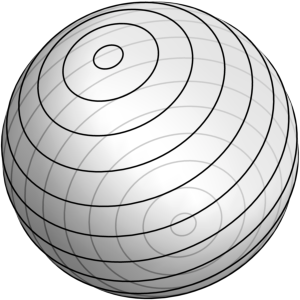
\includegraphics[width=.7\columnwidth]{figures/celestial-ball-1.pdf}
		\caption{Elliptical}
	\end{subfigure}
	\vskip3ex
	\begin{subfigure}{\columnwidth}
		\centering
		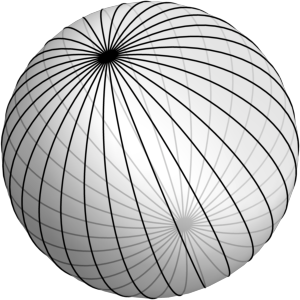
\includegraphics[width=.7\columnwidth]{figures/celestial-ball-2.pdf}
		\caption{Hyperbolic}
	\end{subfigure}
	\vskip3ex
	\begin{subfigure}{\columnwidth}
		\centering
		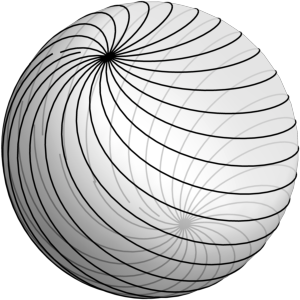
\includegraphics[width=.7\columnwidth]{figures/celestial-ball-3.pdf}
		\caption{Loxodromic}
	\end{subfigure}
	\caption{
		Lorentz transformations on the celestial sphere, taking curves to themselves.
	}
	\label{fig:celestial-balls}
\end{marginfigure}


Elliptical Lorentz transformations are \emph{rotations}, whose rotors are generated by spacelike $2$-blades; hyperbolic transformations are \emph{boosts}, with timelike $2$-blades generators.
Parabolic transformations are sometimes called \emph{null rotations}, and fall in between the previous two, with null $2$-blades as generators.

The final class of loxodromic transformations are a combination of a rotation and a boost where the axis of rotation is parallel with the boost direction (in a particular frame).
A loxodromic generator is \emph{not} a $2$-blade, but a bivector comprising mutually $2$-orthogonal\sidenote{
	in the sense of \cref{def:Δ-orthogonal}, \cref{sec:higher-orthogonal}
} $2$-blades, one timelike and one spacelike.

These can be helpfully visualised by making use of the isomorphism $\SO^+(1,3) \cong \op{Aut}(\CC \cup \set{∞})$ of the Lorentz group with the Möbius group of conformal transformations on the sphere.
An observer undergoing a change of frame will see the celestial sphere transform conformally, as in \cref{fig:celestial-balls}.

\part{General Relativity and Manifold Geometry}
\label{part:2}

hi im content!




\newgeometry{margin=3.5cm}

\bibliography{references}

\end{document}